%% History:
% Pavel Tvrdik (26.12.2004)
%  + initial version for PhD Report
%
% Daniel Sykora (27.01.2005)
%
% Michal Valenta (3.12.2008)
% rada zmen ve formatovani (diky M. Duškovi, J. Holubovi a J. Žďárkovi)
% sjednoceni zdrojoveho kodu pro anglickou, ceskou, bakalarskou a diplomovou praci

% One-page layout: (proof-)reading on display
%%%% \documentclass[11pt,oneside,a4paper]{book}
% Two-page layout: final printing
\documentclass[11pt,twoside,a4paper]{book}   
\renewcommand{\baselinestretch}{1.0} 
%=-=-=-=-=-=-=-=-=-=-=-=--=%
% The user of this template may find useful to have an alternative to these 
% officially suggested packages:
\usepackage[czech, english]{babel}
\usepackage[T1]{fontenc} % pouzije EC fonty 
% pripadne pisete-li cesky, pak lze zkusit take:
% \usepackage[OT1]{fontenc} 
\usepackage[utf8]{inputenc}
%=-=-=-=-=-=-=-=-=-=-=-=--=%
% In case of problems with PDF fonts, one may try to uncomment this line:
%\usepackage{lmodern}
%=-=-=-=-=-=-=-=-=-=-=-=--=%
%=-=-=-=-=-=-=-=-=-=-=-=--=%
% Depending on your particular TeX distribution and version of conversion tools 
% (dvips/dvipdf/ps2pdf), some (advanced | desperate) users may prefer to use 
% different settings.
% Please uncomment the following style and use your CSLaTeX (cslatex/pdfcslatex) 
% to process your work. Note however, this file is in UTF-8 and a conversion to 
% your native encoding may be required. Some settings below depend on babel 
% macros and should also be modified. See \selectlanguage \iflanguage.
%\usepackage{czech}  %%%%%\usepackage[T1]{czech} %%%%[IL2] [T1] [OT1]
%=-=-=-=-=-=-=-=-=-=-=-=--=%

%%%%%%%%%%%%%%%%%%%%%%%%%%%%%%%%%%%%%%%
% Styles required in your work follow %
%%%%%%%%%%%%%%%%%%%%%%%%%%%%%%%%%%%%%%%
\usepackage{graphicx}
%\usepackage{indentfirst} %1. odstavec jako v cestine.

\usepackage{k336_thesis_macros} % specialni makra pro formatovani DP a BP 
 % muzete si vytvorit i sva vlastni v souboru k336_thesis_macros.sty
 % najdete  radu jednoduchych definic, ktere zde ani nejsou pouzity
 % napriklad: 
 % \newcommand{\bfig}{\begin{figure}\begin{center}}
 % \newcommand{\efig}{\end{center}\end{figure}}
 % umoznuje pouzit prikaz \bfig namisto \begin{figure}\begin{center} atd.

\usepackage{enumerate}
\usepackage{listings}

\usepackage{eurosym}

%%%%%%%%%%%%%%%%%%%%%%%%%%%%%%%%%%%%%
% Zvolte jednu z moznosti 
% Choose one of the following options
%%%%%%%%%%%%%%%%%%%%%%%%%%%%%%%%%%%%%
\newcommand\TypeOfWork{Diplomová práce} \typeout{Diplomova prace}
% \newcommand\TypeOfWork{Master's Thesis}   \typeout{Master's Thesis} 
% \newcommand\TypeOfWork{Bakalářská práce}  \typeout{Bakalarska prace}
% \newcommand\TypeOfWork{Bachelor's Project}  \typeout{Bachelor's Project}


%%%%%%%%%%%%%%%%%%%%%%%%%%%%%%%%%%%%%
% Zvolte jednu z moznosti 
% Choose one of the following options
%%%%%%%%%%%%%%%%%%%%%%%%%%%%%%%%%%%%%
% nabidky jsou z: http://www.fel.cvut.cz/cz/education/bk/prehled.html

%\newcommand\StudProgram{Elektrotechnika a informatika, dobíhající, Bakalářský}
%\newcommand\StudProgram{Elektrotechnika a informatika, dobíhající, Magisterský}
% \newcommand\StudProgram{Elektrotechnika a informatika, strukturovaný, Bakalářský}
 \newcommand\StudProgram{Otevřená informatika, strukturovaný, Navazující magisterský}
% \newcommand\StudProgram{Softwarové technologie a management, Bakalářský}
% English study:
% \newcommand\StudProgram{Electrical Engineering and Information Technology}  % bachelor programe
% \newcommand\StudProgram{Electrical Engineering and Information Technology}  %master program


%%%%%%%%%%%%%%%%%%%%%%%%%%%%%%%%%%%%%
% Zvolte jednu z moznosti 
% Choose one of the following options
%%%%%%%%%%%%%%%%%%%%%%%%%%%%%%%%%%%%%
% nabidky jsou z: http://www.fel.cvut.cz/cz/education/bk/prehled.html

%\newcommand\StudBranch{Výpočetní technika}   % pro program EaI bak. (dobihajici i strukt.)
%\newcommand\StudBranch{Výpočetní technika}   % pro prgoram EaI mag. (dobihajici i strukt.) 
\newcommand\StudBranch{Softwarové inženýrství}            %pro STM
%\newcommand\StudBranch{Web a multimedia}                  % pro STM
%\newcommand\StudBranch{Computer Engineering}              % bachelor programe
%\newcommand\StudBranch{Computer Science and Engineering}  % master programe


%%%%%%%%%%%%%%%%%%%%%%%%%%%%%%%%%%%%%%%%%%%%
% Vyplnte nazev prace, autora a vedouciho
% Set up Work Title, Author and Supervisor
%%%%%%%%%%%%%%%%%%%%%%%%%%%%%%%%%%%%%%%%%%%%

\newcommand\WorkTitle{Nástroj pro generování dokumentace vzdálených rozhraní
(API) webových služeb aplikací Java Enterprise Edition}
\newcommand\FirstandFamilyName{Bc.
Tomáš Jiříček} \newcommand\Supervisor{Ing. Tomáš Černý, MSc.}


% Pouzijete-li pdflatex, tak je prijemne, kdyz bude mit vase prace
% funkcni odkazy i v pdf formatu
\usepackage[
pdftitle={\WorkTitle},
pdfauthor={\FirstandFamilyName},
bookmarks=true,
colorlinks=true,
breaklinks=true,
urlcolor=red,
citecolor=blue,
linkcolor=blue,
unicode=true,
]
{hyperref}



% Extension posted by Petr Dlouhy in order for better sources reference (\cite{} command) especially in Czech.
% April 2010
% See comment over \thebibliography command for details.

\usepackage[square, numbers]{natbib}             % sazba pouzite literatury
%\usepackage{url}
%\DeclareUrlCommand\url{\def\UrlLeft{<}\def\UrlRight{>}\urlstyle{tt}}  %rm/sf/tt
%\renewcommand{\emph}[1]{\textsl{#1}}    % melo by byt kurziva nebo sklonene,
\let\oldUrl\url
\renewcommand\url[1]{<\texttt{\oldUrl{#1}}>}




\begin{document}

%%%%%%%%%%%%%%%%%%%%%%%%%%%%%%%%%%%%%
% Zvolte jednu z moznosti 
% Choose one of the following options
%%%%%%%%%%%%%%%%%%%%%%%%%%%%%%%%%%%%%
\selectlanguage{czech}
%\selectlanguage{english} 

% prikaz \typeout vypise vyse uvedena nastaveni v prikazovem okne
% pro pohodlne ladeni prace


\iflanguage{czech}{
	 \typeout{************************************************}
	 \typeout{Zvoleny jazyk: cestina}
	 \typeout{Typ prace: \TypeOfWork}
	 \typeout{Studijni program: \StudProgram}
	 \typeout{Obor: \StudBranch}
	 \typeout{Jmeno: \FirstandFamilyName}
	 \typeout{Nazev prace: \WorkTitle}
	 \typeout{Vedouci prace: \Supervisor}
	 \typeout{***************************************************}
	 \newcommand\Department{Katedra počítačů}
	 \newcommand\Faculty{Fakulta elektrotechnická}
	 \newcommand\University{České vysoké učení technické v Praze}
	 \newcommand\labelSupervisor{Vedoucí práce}
	 \newcommand\labelStudProgram{Studijní program}
	 \newcommand\labelStudBranch{Obor}
}{
	 \typeout{************************************************}
	 \typeout{Language: english}
	 \typeout{Type of Work: \TypeOfWork}
	 \typeout{Study Program: \StudProgram}
	 \typeout{Study Branch: \StudBranch}
	 \typeout{Author: \FirstandFamilyName}
	 \typeout{Title: \WorkTitle}
	 \typeout{Supervisor: \Supervisor}
	 \typeout{***************************************************}
	 \newcommand\Department{Department of Computer Science and Engineering}
	 \newcommand\Faculty{Faculty of Electrical Engineering}
	 \newcommand\University{Czech Technical University in Prague}
	 \newcommand\labelSupervisor{Supervisor}
	 \newcommand\labelStudProgram{Study Programme} 
	 \newcommand\labelStudBranch{Field of Study}
}




%%%%%%%%%%%%%%%%%%%%%%%%%%    Poznamky ke kompletaci prace
% Nasledujici pasaz uzavrenou v {} ve sve praci samozrejme 
% zakomentujte nebo odstrante. 
% Ve vysledne svazane praci bude nahrazena skutecnym 
% oficialnim zadanim vasi prace.
{
\pagenumbering{roman} \cleardoublepage \thispagestyle{empty}
\chapter*{Na tomto místě bude oficiální zadání vaší práce}
\begin{itemize}
\item Toto zadání je podepsané děkanem a vedoucím katedry,
\item musíte si ho vyzvednout na studiijním oddělení Katedry počítačů na Karlově náměstí,
\item v jedné odevzdané práci bude originál tohoto zadání (originál zůstává po obhajobě na katedře),
\item ve druhé bude na stejném místě neověřená kopie tohoto dokumentu (tato se vám vrátí po obhajobě).
\end{itemize}
\newpage
}

%%%%%%%%%%%%%%%%%%%%%%%%%%    Titulni stranka / Title page 

\coverpagestarts

%%%%%%%%%%%%%%%%%%%%%%%%%%%    Podekovani / Acknowledgements 

\acknowledgements
\noindent
Zde můžete napsat své poděkování, pokud chcete a máte komu děkovat.


%%%%%%%%%%%%%%%%%%%%%%%%%%%   Prohlaseni / Declaration 

\declaration{V~Praze dne 10.\,5.\,2015}
%\declaration{In Kořenovice nad Bečvárkou on May 15, 2008}


%%%%%%%%%%%%%%%%%%%%%%%%%%%%    Abstract 
 
\abstractpage

Translation of Czech abstract into English.

% Prace v cestine musi krome abstraktu v anglictine obsahovat i
% abstrakt v cestine.
\vglue60mm

\noindent{\Huge \textbf{Abstrakt}}
\vskip 2.75\baselineskip
% \noindent
S narůstajícím počtem softwarových produktů, které mají potřebu být mezi sebou vzájemně
integrovány vznikl velký tlak na unifikaci rozhraní. Byla proto vytvořena řada protokolů a
technologií, které přinášejí do systémové integrace pravidla a postupy určující jak probíhá
vzdálená komunikace mezi systémy a jak tvořit poskytovatele a klienty takových rozhraní.
Pokud existuje k vystavenému rozhraní odpovídající dokumentace, která umožní
konzumentovi poskytnout všechny potřebné informace o rozhraní, lze poměrně rychle a
jednoduše provést integraci. V opačném případě nekompletní, neaktuální či jinak
nedostačující dokumentace může způsobit nárust nákladů na realizování integrace.

Cílem práce je analyzovat požadavky dokumentace a vytvořit nástroj pro automatické
generování aktuální dokumentace vzdálených rozhraní. S využitím nástroje dojde ke snížení
nákladů potřebných pro tvorbu dokumentace a tím i realizaci systémové integrace.


%%%%%%%%%%%%%%%%%%%%%%%%%%%%%%%%  Obsah / Table of Contents 

\tableofcontents
\addtocontents{toc}{\setcounter{tocdepth}{2}} 


%%%%%%%%%%%%%%%%%%%%%%%%%%%%%%%  Seznam obrazku / List of Figures 

\listoffigures


%%%%%%%%%%%%%%%%%%%%%%%%%%%%%%%  Seznam tabulek / List of Tables

\listoftables

\lstlistoflistings 


%**************************************************************

\mainbodystarts
% horizontalní mezera mezi dvema odstavci
%\parskip=5pt
%11.12.2008 parskip + tolerance
\normalfont
\parskip=0.2\baselineskip plus 0.2\baselineskip minus 0.1\baselineskip

% Odsazeni prvniho radku odstavce resi class book (neaplikuje se na prvni 
% odstavce kapitol, sekci, podsekci atd.) Viz usepackage{indentfirst}.
% Chcete-li selektivne zamezit odsazeni 1. radku nektereho odstavce,
% pouzijte prikaz \noindent.

%**************************************************************

% Pro snadnejsi praci s vetsimi texty je rozumne tyto rozdelit
% do samostatnych souboru nejlepe dle kapitol a tyto potom vkladat
% pomoci prikazu \include{jmeno_souboru.tex} nebo \include{jmeno_souboru}.
% Napr.:
% \include{1_uvod}
% \include{2_teorie}
% atd...

%*****************************************************************************
% \chapter{Úvod}
% \section*{}
Systémová integrace je velmi často skloňovaný pojem. Drtivá většina systémů v dnešní době
není bez integrace schopna fungovat. Schopnost integrace s jinými systémy je žádoucí,
protože čím více se umí software integrovat, tím je flexibilnější. Integrace znamená spojení
menších komponent do vetšího celku. Takový celek potom dokáže efektivně pracovat pomocí
definovaných pravidel pro komunikaci mezi subsytémy. Integraci lze vytvořit na různých
systémových vrstvách.

První počátky integrace sahají do roku 1980, kdy vznikla myšlenka tzv. digitální výroby, která
byla aplikována v továrnách. V devadesátých letech společnosti nakupovaly softwarová řešení
jako je SAP, Oracle ERP, Siebel a další. Tato řešení fungovala dobře jako samostatný
software, vytvořily se kolem nich takzvané informační ostrovy. Ve většině případů každé
řešení produkovalo redundantní data. Ve výsledku při vzniklé změně dat musely být ručně
změněny i v ostatních systémech. Takové řešení bylo těžkopádné a musela přijít změna. Tyto
problémy daly vzniknout rozmachu integrace mezi systémy.

Komunikace mezi komponentami byla často platformově závislá a používaly se pro ni
proprietární protokoly. Postupem času, jak šly informační technologie dopředu a sílil tlak na
vznik technologií umožňujících platformovou nezávislost s otevřenými protokoly pro
komunikaci, jsme ve stavu, kdy máme technologie a standardizované protokoly. S jejich
pomocí vznikají unifikovaná rozhraní systémů, která zjednodušují realizování integrace mezi
softwarovými komponentami.

Protokoly definují jak probíhá komunikace, technologie definují jak vytvářet rozhraní a
klienty k nim, opomíjí se však tvorba, obsah a umístění dokumentace. Přestože poskytovatelé
rozhraní používají jednotné protokoly a technologie, dokumentaci má každý trochu jinou.
Momentálně se můžeme setkat nejčastěji s dokumentací v HTML, dokumentech
kancelářských balíků či PDF dokumentech. Taková dokumentace je tvořena ručně a má řadu
nevýhod. Při její tvorbě může být zanesena chyba, dokumentace nemusí být aktuální a nemusí
odpovídat popisovanému rozhraní. Dále usí existovat člověk, který bude za dokumentaci
zodpovědný. Provádět integraci se systémem mající neodpovídající dokumentaci může
prodloužit dobu integrace a tím vzrostou náklady.

Cílem diplomové práce je navrhnout, implementovat a otestovat nástroj pro automatické
generování dokumentace vzdálených rozhraní. Nástroj by měl odstranit problémy s tvorbou
dokumentace, protože proces její tvorby nebude zahrnovat lidský element a bude zajištěno,
aby se dokumentace aktualizovala vždy se změnou rozhraní. 

\end{document}
\chapter{Úvod} 
% \section*{}
Systémová integrace je velmi často skloňovaný pojem. Drtivá většina systémů v dnešní době
není bez integrace schopna fungovat. Schopnost integrace s jinými systémy je žádoucí,
protože čím více se umí software integrovat, tím je flexibilnější. Integrace znamená spojení
menších komponent do vetšího celku. Takový celek potom dokáže efektivně pracovat pomocí
definovaných pravidel pro komunikaci mezi subsytémy. Integraci lze vytvořit na různých
systémových vrstvách.

První počátky integrace sahají do roku 1980, kdy vznikla myšlenka tzv. digitální výroby, která
byla aplikována v továrnách. V devadesátých letech společnosti nakupovaly softwarová řešení
jako je SAP, Oracle ERP, Siebel a další. Tato řešení fungovala dobře jako samostatný
software, vytvořily se kolem nich takzvané informační ostrovy. Ve většině případů každé
řešení produkovalo redundantní data. Ve výsledku při vzniklé změně dat musely být ručně
změněny i v ostatních systémech. Takové řešení bylo těžkopádné a musela přijít změna. Tyto
problémy daly vzniknout rozmachu integrace mezi systémy.

Komunikace mezi komponentami byla často platformově závislá a používaly se pro ni
proprietární protokoly. Postupem času, jak šly informační technologie dopředu a sílil tlak na
vznik technologií umožňujících platformovou nezávislost s otevřenými protokoly pro
komunikaci, jsme ve stavu, kdy máme technologie a standardizované protokoly. S jejich
pomocí vznikají unifikovaná rozhraní systémů, která zjednodušují realizování integrace mezi
softwarovými komponentami.

Protokoly definují jak probíhá komunikace, technologie definují jak vytvářet rozhraní a
klienty k nim, opomíjí se však tvorba, obsah a umístění dokumentace. Přestože poskytovatelé
rozhraní používají jednotné protokoly a technologie, dokumentaci má každý trochu jinou.
Momentálně se můžeme setkat nejčastěji s dokumentací v HTML, dokumentech
kancelářských balíků či PDF dokumentech. Taková dokumentace je tvořena ručně a má řadu
nevýhod. Při její tvorbě může být zanesena chyba, dokumentace nemusí být aktuální a nemusí
odpovídat popisovanému rozhraní. Dále usí existovat člověk, který bude za dokumentaci
zodpovědný. Provádět integraci se systémem mající neodpovídající dokumentaci může
prodloužit dobu integrace a tím vzrostou náklady.

Cílem diplomové práce je navrhnout, implementovat a otestovat nástroj pro automatické
generování dokumentace vzdálených rozhraní. Nástroj by měl odstranit problémy s tvorbou
dokumentace, protože proces její tvorby nebude zahrnovat lidský element a bude zajištěno,
aby se dokumentace aktualizovala vždy se změnou rozhraní.

\chapter{Analýza}
\section{Specifikace technologií pro vzdálená rozhraní}
Způsobů jak na platformě Java Enterprise Edition vzdáleně komunikovat mezi systémy přes
internet je několik. V současné době se pro integraci nejvíce používají SOAP Web Services
(WS), Representational State Transfer (REST) a Java Message Service (JMS). Dalšími
způsoby vzdálené komunikace jsou například
Remote Method Invocation (RMI) nebo
Common Object Request Broker Architecture (CORBA). Tato práce se zabývá prvními třemi
zmíněnými systémy.


\subsection{Web Services}
Web Services jsou založeny na technologiích XML, WSDL a SOAP. Jsou pro ně
definovány čtyři hlavní protokoly.

\subsubsection{Transportní protokol (Transport Protocol)}
Přes transportní protokol jsou posílány zprávy po síti. Jako transportní protokol se nejčastěji
využívá HTTP, SMTP a FTP. V prostředí Javy lze použít JMS, což je API pro posílání zpráv.
Nejedná se o protokol jako v předchozích případech. Každý implementátor JMS si může
vytvořit svůj protokol pro posílání zpráv, který nazýváme „wire protocol“. Je důležité, aby
různé implementace dokázaly mezi sebou komunikovat. Praxe však ukazuje, že ne všechny
implementace jsou mezi sebou plně kompatibilní.

\subsubsection{Protokol zpráv (Messaging Protocol)}

\begin{figure}[h]
\begin{center}
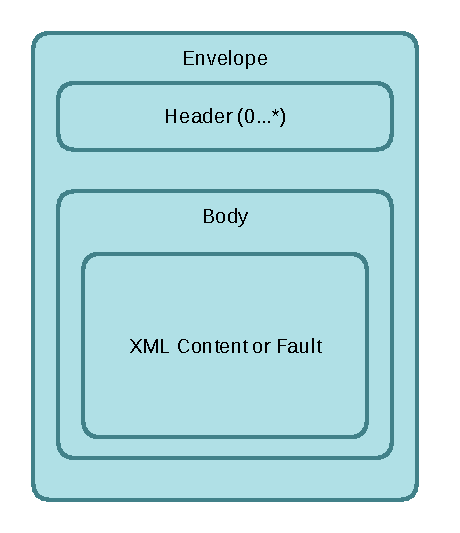
\includegraphics[width=7cm]{images-pdf/soap.pdf} 
\caption{SOAP zpráva}
\label{fig:logo}
\end{center}
\end{figure}

Protokol zpráv je zodpovědný za zakódování a dekódování zprávy do, resp. z XML-like
formátu. Nejčastěji se užívá protokol SOAP (Simple Access Object Protocol). SOAP udává,
jak bude vypadat přenášená zpráva, která se skládá ze čtyř hlavních částí:

\begin{itemize}
\item Envelope – kořenový element SOAP zprávy, který je povinný a definuje, že jeho
obsahem je SOAP zpráva.

\item Header –
volitelný element, který se používá pro přidání nové funkcionality a
vlastností, jakou může být například autentizace. Ve zprávě je povoleno použít více
těchto elementů. Pokud je header ve zprávě přítomen, musí být umístěn jako první
child element elementu envelope.
 
\item Body – povinný element, který obsahuje přenášená data nazývána „payload“. Body
musí být uvnitř elementu envelope a následuje až za elementy message. Sémantika
obsahu v elementu body je definována v XML Schema.

\item Fault – tento element je umístěn v elementu body. Ve zprávě se objevuje, pokud je
nutné poslat informaci o vzniklé chybě. Fault má definováno, jak má informace o
chybě vypadat a obsahuje následující subelementy:

\begin{itemize}
  \item faultCode
  \item faultString
  \item faultActor
  \item detail.
\end{itemize}
\end{itemize}

\subsubsection{Protokol popisující službu (Description Protocol)}

\begin{figure}[h]
\begin{center}
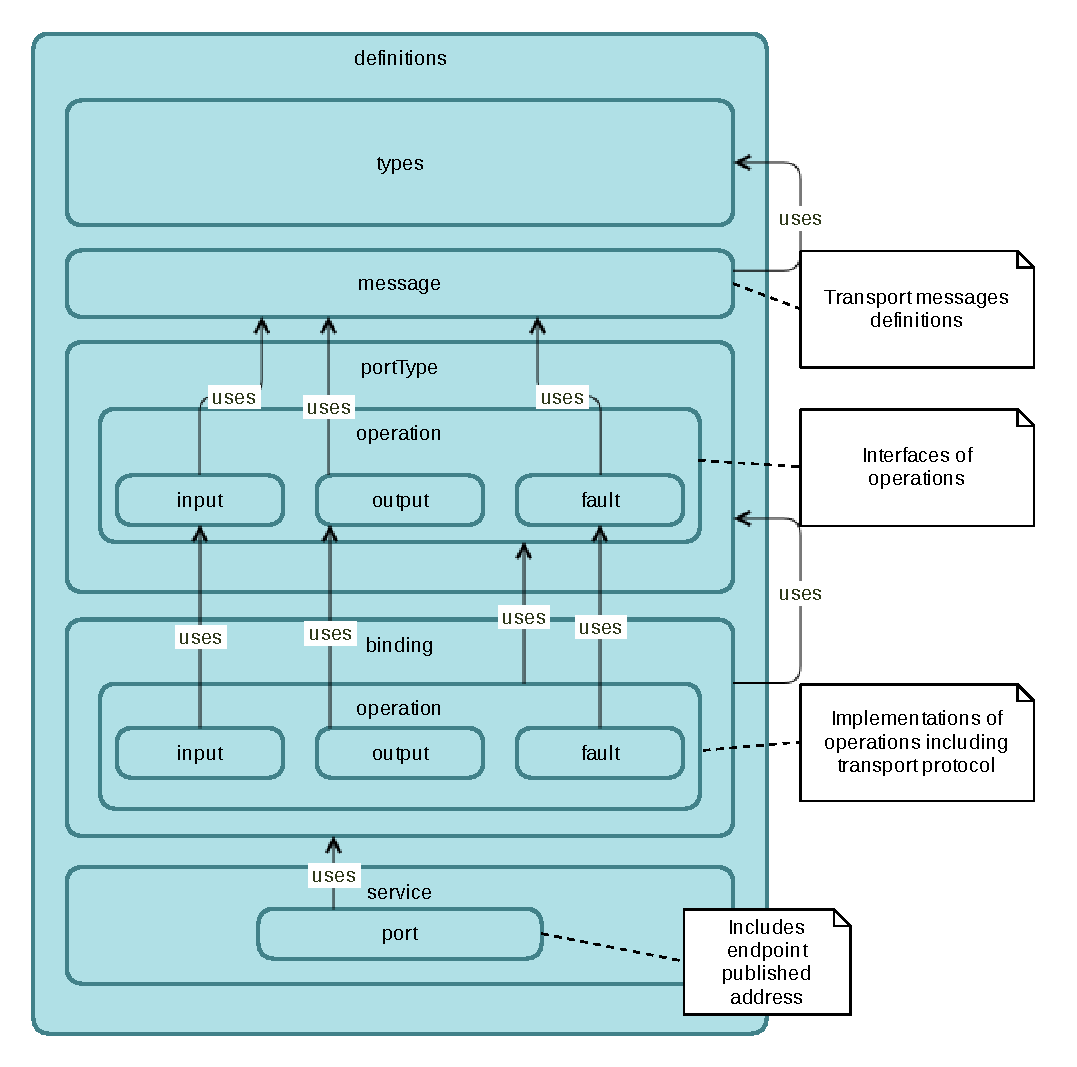
\includegraphics[width=12cm]{images-pdf/wsdl.pdf} 
\caption{Struktura WSDL}
\label{fig:logo}
\end{center}
\end{figure}

Protokol description popisuje veřejné rozhraní dané WS. Typicky se používá WSDL (Web
Service Description Protocol), což je XML-based protokol. WSDL definuje, jak ke službě
přistupovat a jaké metody můžeme na službě volat. V tomto protokolu jsou dále zaneseny
například informace, jaké má metoda parametry, jaké návratové hodnoty a jaké mohou nastat
faulty při volání metody.

Kořenový element WSDL dokumentu se jmenuje definitions. Schéma elementu je na 2.
Definitons formuluje název webové služby a deklaruje jmenné prostory, které nazýváme
„namespacy“. Uvnitř definitions je několik přímých elementů:

\begin{itemize}
  \item Types - element obsahující všechny datové typy, které se mohou přenášet. Datové
typy jsou zapsány v XML Schema.

  \item Message – značí abstrakci přenášené zprávy. Těchto elementů bývá zpravidla více,
protože pro jednu metodu, která má mít vstup, výstup a fault, musí existovat tři tyto
elementy. Části elementu message se budou skládat z datových typů definovaných v
 elementu types. 

  \item PortType – jedná se o abstraktní množinu operací k jednomu nebo více endpointům,
které mohou být volány. Těmto operacím se potom v elementu binding nastavuje
transportní protokol.

  \begin{itemize}
    \item Operation - přímý potomek elementu portType, který lze přirovnat k metodě v
klasických programovacích jazycích jako je například Java či C. V tomto
elementu je definováno jméno metody, input message, output message a fault.
Části input, output a fault se odkazují na definice v elementech message.

  \end{itemize}
  \item Binding – tento element definuje pro každý portType konkrétní datové typy, operace
a protokol.

  \item Service - poslední přímý potomek kořenového elementu. Uvnitř něj je definován
seznam endpointů. Binding služby je zde mapován na port.

  \begin{itemize}
    \item Port - přímý potomek elementu service. Port je kombinací bindingu a síťové
adresy, na které je služba dostupná.

  \end{itemize}
\end{itemize}

\subsubsection{Protokol pro objevování služeb (Discovery Protocol)}
Protokol pro objevování služeb je XML-based registr, díky němuž mohou být po celém
internetu shromažďovány informace o webových službách. Umožňuje zaregistrování webové
služby a jejich procházení v daném registru, který nazýváme UDDI. V tomto registru je
možné získat dokument popisující službu (WSDL) a její metadata.

\begin{figure}[h]
\begin{center}
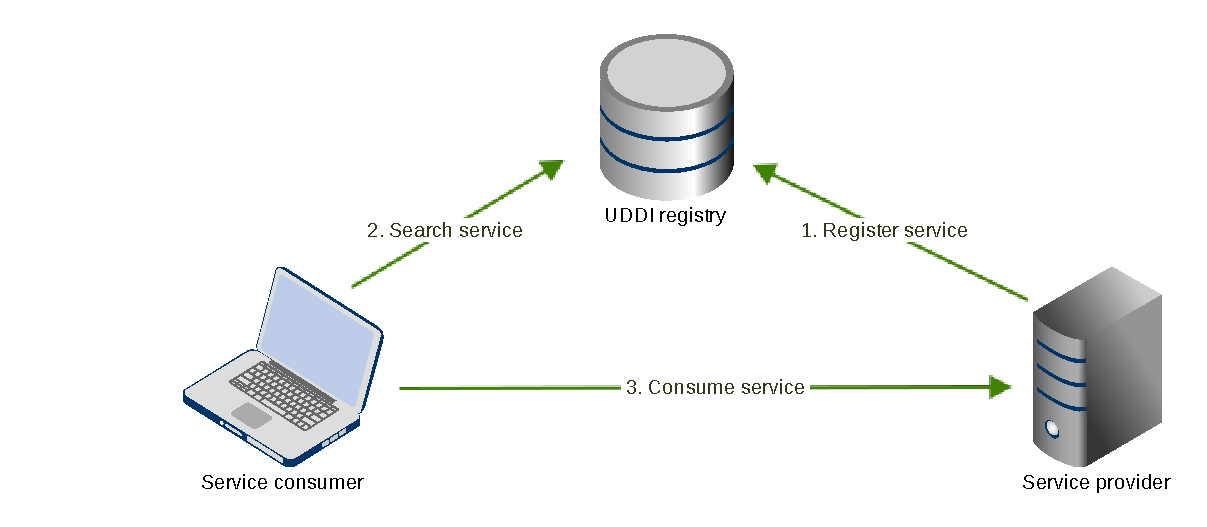
\includegraphics[width=13cm]{images-pdf/uddi.pdf} 
\caption{Discovery protocol}
\label{fig:logo}
\end{center}
\end{figure}

Informace o určité službě jsou obsaženy napříč třemi komponentami, které UDDI obsahuje -
v každé jsou informace jiného charakteru:

\begin{itemize}
  \item Bílé stránky - obsahují informace o poskytovateli služby, jako je například jméno
firmy, podrobnosti o firmě či kontakt do firmy.

  \item Žluté stránky - obsahují zařazení služby či poskytovatele do taxonomie, která může
být například geografická. Dalšími typy taxonomie jsou Standard Industrial
Classification či United Nations Standard Products and Services Code.

  \item Zelené stránky - v této komponentě nalezneme technické informace o službě. V
zelených stránkách lze zjistit, na jaké adrese je služba dostupná, service binding nebo
parametry či odkazy na specifikaci rozhraní. Mohou zde být informace s kontaktními
údaji na službu s určitým bindingem. Pokud má totiž služba více bindingů, bude mít i
více záznamů v zelených stránkách.

\end{itemize}

\subsection{REST Web Services}

Na rozdíl od klasických WS není pro REST služby definovaný žádný protokol. Jedná
se o architektonický styl pro návrh aplikací a název vznikl jako zkratka z  Representational State Transfer. REST služby jsou orientovány na zdroje (resources) a jsou aplikací architektury webu na architekturu webových aplikací. 

Aplikaci můžeme nazvat REST, pokud bude splňovat následující omezení:

\textbf{\textit{Klient-server}}

Aplikace je postavena na modelu, kde je klient oddělen od serveru. Server si nepamatuje
stavy, ve kterých se klienti nachází. Klienti a servery mohou být vyvíjeni paralelně, protože
mají definované rozhraní mezi sebou. Další výhodou je, že mohou být nahrazeni za jiné
klienty nebo servery.

\textbf{\textit{Bezstavová komunikace}}

Veškerý stav, ve kterém se aplikace nachází si uchovává klient. Bezstavová aplikace se velmi
dobře škáluje. Na druhou stranu musí každý dotaz obsahovat veškeré informace o stavu
aplikace vůči klientovi. Pokud klient poslal požadavek, který ještě nebyl vyřízen, nachází se
klient v tzv. stavu přechodu.

\textbf{\textit{Cache}}

Stejně jako World Wide Web, klienti mohou kešovat odpovědi. Odpovědi musí být
definovány jako kešovatelné nebo nekešovatelné. Dobře spravované kešování aplikace
pomáhá k lepšímu výkonu, protože se v mnoha případech nemusí posílat požadavek až do
aplikace na serveru.

\textbf{\textit{Vrstvený systém}}

Vrstvený systém dovolí mezi server a klienta vložit systém jiný, kterým může být cache nebo
loadbalancer, aniž by klient pocítil změnu. Klient nemá k dispozici informaci, se kterým
systémem komunikuje.

\textbf{\textit{Jednotné rozhraní}}

Jednotným rozhraním je myšleno použití malé množiny dobře definovaných metod k
manipulaci se zdroji. K tomuto rozhraní se vztahují následující omezení:

\begin{itemize}
  \item HATEOAS (hypermedia as the engine of application state) – klienti mohou přejít
dynamicky do jiného stavu v aplikaci přes hypermedia poslané serverem v předchozí
odpovědi. Jinými slovy, odpověď od serveru obsahuje hyperlinky, na které může klient
přejít, aby se dostal do jiného stavu v aplikaci.
  \item Adresovatelné zdroje – každý zdroj poskytující informace a data musí být
jednoznačně identifikovaný svou URI (Uniform Resource Identifier).
\item Manipulace se zdrojem a jejich reprezentacemi – pokud se klient nachází na
nějakém zdroji, může s ním provádět operace modifikace či smazání.
\item Orientace na reprezentaci – u jedné URI lze nastavit, aby dokázala použít odlišné
formáty dat, protože ne všechny platformy užívají stejný formát. Například webový
prohlížeč používá HTML a JavaScript, který potřebuje JSON. Java aplikace může
vyžadovat XML.
\end{itemize}

\textbf{\textit{Kód na vyžádání (volitelné)}}

Server může poslat na klienta spustitelný kód, který rozšiřuje funkčnost. Takový kód může
být ve formě JavaScriptu nebo třeba Java appletu.

\subsubsection{Svázání RESTu s protokolem HTTP}

REST nemá definovaný žádný protokol, avšak ve většině případů, kdy se zmiňujeme o
RESTu, máme na mysli REST přes HTTP. Webové aplikace ve webových prohlížečích 
využívají pouze nepatrnou část vlastností HTTP. Aplikace založené na klasických WS
používají HTTP protokol striktně jako transportní vrstvu především kvůli průchodu přes
firewally a využívají tak také jen malou část HTTP.

\begin{figure}[h]
\begin{center}
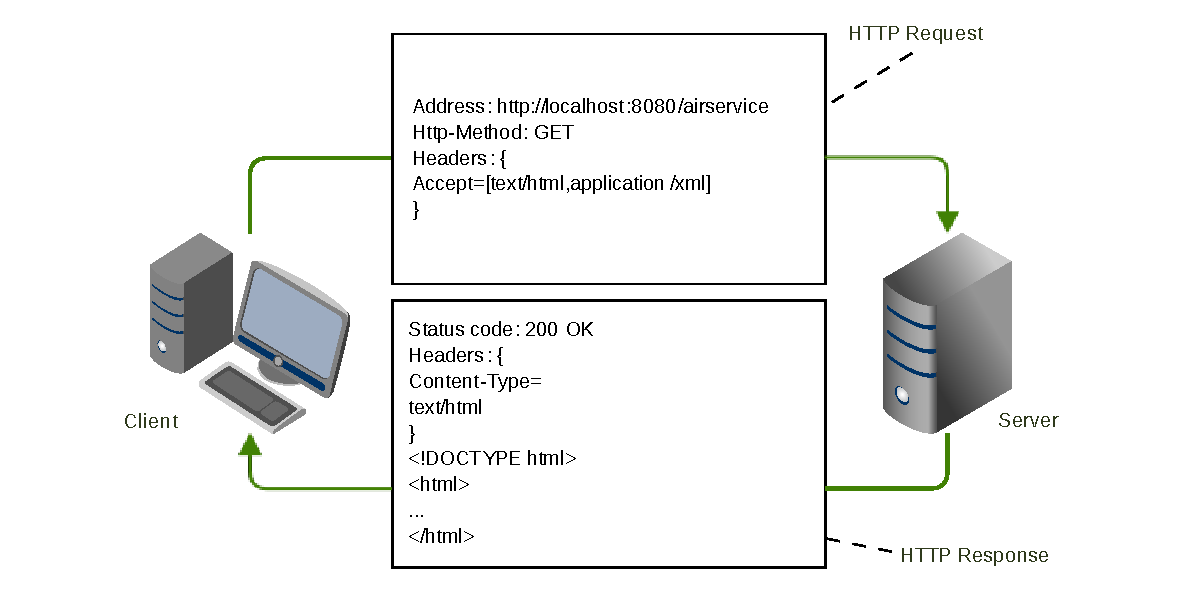
\includegraphics[width=13cm]{images-pdf/http.pdf}
\caption{Ukázka komunikace přes HTTP}
\label{fig:logo}
\end{center}
\end{figure}

HTTP je aktuálně velmi bohatý aplikační protokol, poskytující množství zajímavých a
užitečných schopností. Podmínkou pro psaní RESTful aplikací je velmi dobrá znalost HTTP
protokolu. HTTP je protokol s určitými vlastnostmi (synchronní, požadavek/odpověď,
aplikační, síťový) používaný pro distribuované, spolupracující systémy. Jedná se o primární
protokol používaný na webu, který je velmi jednoduchý - klient posílá požadavek složený z
názvu HTTP metody, lokaci zdroje, hlavičky a volitelně z těla požadavku, které může
obsahovat cokoliv. Nejčastěji se však pro tělo požadavku používá reprezentace dat v JSON,
XML, HTML nebo plain text.

\section{Rešerše generování vzdáleného API na platformě Java EE}

\subsection{Specifikace JAX-WS}
Specifikace JAX-WS je standardizovaná technologie pro tvorbu Web Services na platformě
Java. JAX-WS API skrývá aplikačnímu vývojáři svou komplexitu. Na serverové straně je
třeba definovat interface a v něm metody, které se budou mapovat na operace v endpointu.

Specifikace nenutí, aby byly SOAP zprávy generovány a parsovány programově, protože
JAX-WS runtime systém převádí zprávy na Java objekty a obráceně za programátora. V
některých situacích se však může stát, že je nutné zprávu generovat či parsovat ručně, což ale
JAX-WS umí, a to na různých úrovních abstrakce.

\subsubsection{Web Service endpoint implementation}
Výchozím bodem pro tvorbu JAX-WS webové služby je třída mající anotaci @WebService,
která je definována jako web service endpoint. Service endpoint interface nebo service
endpoint implementation (SEI) je Java interface či třída deklarující metody, které může klient
konzumovat na webové službě. Při tvorbě endpointu není povinné mít interface, protože třída
implicitně definuje service endpoint interface. Pokud přeci jenom chceme oddělit
funkcionalitu od rozhraní, je nutné, kromě toho, aby třída implementovala interface, nastavit v
anotaci @WebService v elementu endpointInterface celý název interfacu, tedy i s packagem.
Název služby (service name) lze získat z elementu serviceName anotace @WebService a
pokud je hodnota elementu prázdná, použije se název implementující třídy s příponou
„Service“.

Pokud třída implicitně definuje SEI, jako webové operace budou namapovány metody s
modifikátorem public, které splňují následující:
\begin{itemize}
  \item Metoda je anotována s @WebMethod, jejíž element exclude je roven hodnotě false.
False je defaultní hodnota, tudíž není povinné element specifikovat.
  \item Metoda není anotována s @WebMethod anotací, ale její deklarující třída má anotaci
@WebService.
\end{itemize}

Pro mapovací účely u implicitního SEI jsou mapovány stejné anotace jako u implementace
webové služby a jejích metod. Pokud nastane situace, že u třídy anotované s @WebService
chceme public metodu vynechat z mapování na WS operaci a máme SEI definované
implicitně, musíme přidat k metodě anotaci @WebMethod a element exclude nastavit na true.
Pro mapovací účely musí být třída top-level class nebo statická inner class. Třída anotovaná
@WebService musí mít defaultní public konstruktor.

\subsubsection{Web Service endpoint interface}
Java service endpoint interface (SEI) je mapováno na wsdl:portType element. SEI je Java
interface, který splňuje následující omezení:

\begin{itemize}
  \item Musí být anotován s @WebService.
  \item V @WebService smí být vyplněn pouze element targetNamespace.
  \item Jakákoliv metoda může být anotována s @WebMethod.
  \item Pokud je u metody použita anotace @WebMethod, nesmí obsahovat element exclude s
hodnotou true.
  \item Všechny parametry a návratové typy musí být kompatibilní s JAXB 2.0 specifikací.
\end{itemize}

WSDL 1.1 nedefinuje standardní formu dědičnosti pro wsdl:portType elementy. Jediná
povolená dědičnost je dědění Java metod s JAX-WS anotacemi. I když jsou metody
definovány v jiném interfacu než v SEI, je s nimi zacházeno jako kdyby byly definovány
uvnitř SEI.

\subsubsection{Metoda}

Každá public metoda v SEI nemající anotaci @WebMethod s elementem exclude nastaven na
true je mapována na wsdl:operation element v korespondujícím wsdl:portType.

Jméno WS operace je mapováno z elementu name v anotaci @WebMethod a pokud je
element nespecifikován, použije se jméno Java metody. Element name se používá k řešení
jmenných konfliktů, když existuje více potencionálních WS operací se stejným názvem.

Web Services definují dva druhy metod, jimiž jsou one-way a two-way. One-way mají vstup,
ale neprodukují žádný výstup. Two-way mají vstup a produkují výstup. Defaultně jsou
všechny metody mapovány na operace typu two-way. Pro definování operace one-way stačí
metodu anotovat s @OneWay. One-way operace ve WSDL mají definován element
wsdl:input, definující vstupní parametry. Pro operace two-way je navíc definován element
wsdl:output za předpokladu, že Java metoda nevrací typ void. U two-way jsou definovány
wsdl:fault elementy v rozsahu nula až vícekrát. Fault je mapován z výjimek definovaných v
metodě.

One-way metoda musí splňovat určitá kritéria. Pouze metody s návratovým typem void,
nemající parametr implementující Holder, a které nevyhazují kontrolované výjimky, mohou,
nikoliv musí, být typu one-way.

Elementy wsdl:input, wsdl:output a wsdl:fault jsou asociovány s elementy wsdl:message,
které definují přenášené zprávy. Hodnota atributu name elementu wsdl:message není nijak
důležitá a proto se používá hodnota jména operace pro příchozí zprávy a hodnota jména
operace zřetězená s „Response“ pro odchozí zprávy. U zpráv typu fault se použije pro
hodnotu atributu název Java výjimky, pokud není specifikováno jinak v anotaci @WebFault u
metody.

Pro každý element wsdl:message lze definovat Document styl nebo RPC styl. V Javě se dá
styl zpráv nakonfigurovat jak pro celý SEI, tak jednotlivě pro každou metodu. Slouží k tomu
anotace @SOAPBinding a element style.

\subsubsection{Parametry a návratové typy}

Parametry a návratový typ Java metody jsou mapovány buď na zprávy nebo na deklarace
globálních elementů. Pro customizaci mapování parametru na zprávu je určena anotace
@WebParam a pro stejný účel slouží anotace @WebResult u návratového typu. Parametry
mohou být mapovány na komponenty pro příchozí zprávy, odchozí zprávy nebo pro oboje.
Mapování záleží na klasifikaci parametru. Parametr může být namapován jako SOAP
hlavička ve zprávě nastavením elementu header na true v anotaci @WebParam. Element
header v anotaci @WebResult může být použit pro vložení výsledku do SOAP hlavičky.

Parametry a návratové typy jsou rozděleny na tři módy podle toho, ve kterých zprávách se
vyskytují.

\begin{itemize}
  \item In – hodnota je přenášena ve zprávě z klienta na SEI, ale není přenášena zpět.
  \item Out – hodnota je přenášena ve zprávě z SEI ke klientovi, ale není přenášena zpět.
  \item In/out – hodnota je přenášena z klienta na SEI a zpět ke klientovi.
\end{itemize}

Návratový typ je vždycky mód out. U parametrů, jejichž typ je obalen třídou Holder
(Holder<T>), je možno nastavit mód in/out nebo out. U ostatních parametrů je vždy použit
mód in. Při obalení parametrů do Holder můžeme docílit funkcionality, kterou Java neumí a to
je vracet více hodnot z jedné metody. V anotaci @WebParam se elementem mode nastavuje
mód.

\subsubsection{Serializace dat}

Pro definici serializace Java typů do SOAP zprávy je použita anotace @SOAPBinding, kterou
je možno použít u třídy nebo metody. Anotace @SOAPBinding má tři elementy:

\begin{table}[h]
\begin{center}
\begin{tabular}{|c|l|l|}
\hline
\textbf{Element} & \textbf{Výčet hodnot} \\
\hline
Style & DOCUMENT, RPC \\
\hline
Use & LITERAL, ENCODING \\
\hline
ParameterStyle & WRAPPER, BARE \\
\hline
\end{tabular}
\end{center}
\caption{Ukázka tabulky}
\label{tab:tab1}
\end{table}

Kombinováním těchto tří elementů lze vytvářet odlišné struktury zpráv se stejnými nosnými
daty. Struktura zprávy je určena na základě zvolených hodnot v elementech @SOAPBinding.

\begin{enumerate}
  \item Style
  	\begin{enumerate}[(a)]
  	  \item DOCUMENT - obsah SOAP body bude XML dokument, který bude
možno validovat vůči předdefinovanému XML Schema dokumentu.
  	  \item RPC - SOAP body bude obsahovat XML reprezentaci volání metody.
Použije se přitom jméno metody jako hlavní element a jako potomci budou
parametry metody a návratová hodnota.
	\end{enumerate}
  \item Use
	\begin{enumerate}[(a)]
	  \item ENCODING – udává, jak jsou hodnoty zakódovány do XML formátu.
SOAP ENCODING je rozšíření SOAP Frameworku a nabízí pravidla, jak
konvertovat jakákoliv data z SOAP datového modelu do XML formátu.
	  \item LITERAL - definuje, že data jsou serializována podle XML Schema.
	\end{enumerate}
  \item ParameterStyle
	\begin{enumerate}[(a)]
	  \item WRAPPED - říká, že zpráva bude zabalena ještě do jednoho elementu.
	  \item BARE - udává neobalování hodnot do jednoho hlavního předka.
	\end{enumerate}
\end{enumerate}

Přístup DOCUMENT/LITERAL je jednodušší přístup, protože se jednoduše spoléháme na
validaci zprávy vůči XML Schema.

Tvorba XML Schema z Java typů je definována pomocí JAXB. Pomocí tohoto mapování
JAX-WS generuje do WSDL datové typy, které jsou užívány v elementech message. Jsou
podporovány tři styly mapování: document wrapped, document bare a RPC. Styly se liší v
XML Schema konstrukcích.

\textbf{\textit{Document wrapped}}

Document wrapped je definován v anotaci @SOPABinding s následujícími vlastnostmi:

\begin{itemize}
  \item style – DOCUMENT,
  \item use – LITERAL,
  \item parameterStyle – WRAPPED.
\end{itemize}

Pro parametry se vytvoří wrapper, do kterého budou vygenerované typy umístěny a pro
návratový typ se vytvoří druhý wrapper. Jejich vlastnosti se dají upravit v anotacích
@RequestWrapper a @ResponseWrapper. Zde přicházejí do popředí módy (in, out, in/out):

\begin{itemize}
  \item Parametr s módem in je mapován jako potomek globálního elementu request beany.
  \item Parametr s definovaným out nebo návratová hodnota jsou mapováni jako potomci
response beany.
  \item Parametr s módem in/out je mapován jako potomek request beany i response beany.
\end{itemize}

\textbf{\textit{Document bare}}

Styl document bare je definován v anotaci @SOAPBinding s následujícími vlastnostmi:

\begin{itemize}
  \item style – DOCUMENT,
  \item use – LITERAL,
  \item parameterStyle – BARE.
\end{itemize}

Při aplikaci document bare jsou na metodu kladeny tyto požadavky:

\begin{itemize}
  \item Metoda musí mít maximálně jeden parametr in nebo in/out, který není mapován na
hlavičku.
  \item Pokud má návratový typ jiný než void, nesmí mít in/out a out parametry, které nejsou
mapovány na hlavičky.
  \item Pokud má návratový typ void, může mít maximálně jeden parametr in/out
nebo out, který není mapován na hlavičku.
\end{itemize}

Globální deklarace elementu je vygenerována pro vstupní typ metody a analogicky pro
výstupní typ metody.

\textbf{\textit{Styl RPC}}

Styl RPC je definován v anotaci @SOAPBinding s následujícími vlastnostmi:

\begin{itemize}
  \item style – RPC,
  \item use – LITERAL,
  \item parameterStyle – WRAPPED.
\end{itemize}

Java typy pro parametry in, in/out, out a návratové typy jsou mapovány na XML Schema typy
s použitím JAXB. Pro každý parametr metody a návratový typ je vytvořen ve WSDL
dokumentu element part, který je použit v elementu message. Při použití RPC stylu nesmí být
posílány null hodnoty.

\subsection{Specifikace JAX-RS}

Specifikace JAX-RS byla vytvořena za účelem zjednodušení vývoje REST služeb. Použitím
JAX-RS je webový resource implementován jako resource třída a požadavky jsou
obsluhovány resource metodami.

\subsubsection{Resource třída}

Resource třída je Java třída používající JAX-RS anotace k implementaci konkrétního
webového resource. Musí splňovat požadavek na POJO třídu a zároveň musí mít alespoň
jednu metodu s anotací @Path nebo s anotací obsahující request method designator. Pokud
není explicitně změněno, nová instance resource třídy je vytvořena pokaždé, když přijde
požadavek na webový resource, jenž třída implementuje. Implementace JAX-RS může kromě
lifecyclu per-request poskytovat další volby lifecyclu. Speciální resource třídou je root
resource třída, která jak její název napovídá je kořenová. Aby se resource třída mohla stát
kořenovou, musí obsahovat anotaci @Path s URI, na které bude tato root resource třída
zaregistrována a kde bude vyřizovat požadavky.

\subsubsection{Konstruktor}

Root resource třída je instanciovaná JAX-RS runtimem a musí mít konstruktor s
modifikátorem public, který může být bezparametrický nebo parametrický. Může obsahovat
takové parametry, aby je JAX-RS runtime byl schopen předat konstruktoru. Jako parametry
může konstruktor obsahovat ty, které jsou anotovány @Context, @HeaderParam,
@CookieParam, @MatrixParam, @QueryParam a @PathParam. Pokud je obsaženo více
public konstruktorů, použije se ten, který obsahuje nejvíce parametrů. Při shodě počtu
parametrů dvou konstruktorů není pořadí jednoznačně určeno a implementace JAX-RS si
mohu zvolit, který z nich použijí, zároveň by však měly generovat varování o této
víceznačnosti. Non-root resource třída je instanciovaná aplikačním kódem a nepotřebuje výše
popisovaný public konstruktor.

\subsubsection{Atributy}
\label{ch:atributy}

Při vytváření instance resource třídy lze naplnit její atributy konstruktorem nebo setter
metodami. Pokud má atribut modifikátor public, lze přidat anotace přímo k atributu. Anotace
jsou stejné u všech tří zmíněných přístupů plnění hodnot - @Context, @HeaderParam,
@CookieParam, @MatrixParam, @QueryParam a @PathParam. Protože injektování probíhá
při tvorbě objektu, použití těchto anotací (s výjimkou @Context) v resource třídě u
konstruktoru a při nastavování atributů je podporováno pouze u per-request lifecycle. Objekty
vrácené pomocí sub-resource lokátoru se inicializují programově přímo v kódu, nejsou tedy
ve správě JAX-RS runtime.

Typy, pro které mohou být použity anotace @HeaderParam, @CookieParam, @MatrixParam,
@QueryParam a @PathParam, musí splňovat jednu z následujících podmínek:

\begin{enumerate}
  \item Typy, pro které je ParamConverter definován pomocí registrace
  ParamConverterProvideru.
  \item Primitivní typy.
  \item Typy mající konstruktor, který obsahuje jeden parametr typu String.
  \item Typy mající statickou metodu pojmenovanou valueOf nebo fromString s jedním
parametrem typu String a návratovou hodnotou vracející instanci daného typu. Pokud
typ není enum, musí být při výskytu obou metod současně upřednostněna valeuOf. V
případě enum má přednost fromString metoda.
  \item List<T>, Set<T> nebo SortedSet<T>, kde T vyhovuje bodu 3 nebo 4.
\end{enumerate}

Anotace @DefaultValue může být použita pro případ, kdy atribut nedostane žádnou hodnotu.
Anotace přijímá hodnotu jako String a ten je poté převáděn do požadované podoby pomocí
kroků 1 – 5 výše.

\subsubsection{Resource metoda}
\label{subsec:resource-metoda}

Resource metoda je metoda obsluhující požadavek, který přišel na resource třídu. Tato metoda
musí mít anotaci request method designatoru. Taková anotace má anotaci @HttpMethod a
JAX-RS definuje množinu request method designátorů pro obecně definované HTTP metody.
Jejich anotace jsou následující @GET, @POST, @PUT, @DELETE, @HEAD, @OPTIONS.
Lze si zadefinovat designator pro vlastní HTTP metodu tím, že se vytvoří anotace mající
anotaci @HttpMethod. Pouze metody, které mají modifikátor přístupu public, mohou být
považovány jako resource metody.

Po invokaci resource metody jsou parametry anotované @Context, @HeaderParam,
@CookieParam, @MatrixParam, @QueryParam, @PathParam a @FormParam mapovány z
požadavku podle sémantiky anotace. Podobně jako u atributů je zde možno použít anotaci
@DefaultValue. Parametr nemající výše uvedenou anotaci je označován jako entity parametr
a je mapován z těla požadavku. Za převody mezi tělem požadavku a Java typem jsou
zodpovědní entity provideři. Resource metoda může mít maximálně jeden entity parametr.

Resource metoda může vracet návratový typ void, Response, GenericEntity nebo jiný Java
typ. Tyto typy jsou mapovány do těla odpovědi následovně:

\begin{itemize}
  \item Void – prázdné tělo odpovědi se status kódem 204.
  \item Response – tělo odpovědi je naplněno z entity property objektu typu Response se
status kódem specifikovaným ve status property objektu typu Response. Pokud je
návratová hodnota null, status kód bude 204. Při non-null entity property v Response a
nespecifikovaném statusu je status nastaven na 200. Při null entity property je status
nastaven na 204.
  \item GenericEntity – tělo odpovědi je naplněno z entity property objektu typu
GenericEntity. Při null těle odpovědi je status 204, při non-null 200.
  \item Ostatní – tělo odpovědi je přímo mapováno z instance, která se vrací.
Pokud je vrácena instance anonymní vnitřní třídy, je použit její předek. Při null je status 204,
jinak 200.
\end{itemize}

Metody, které potřebují posílat více metadat než jen tělo odpovědi a status kód, by měly
vracet instanci třídy Response.

\begin{table}
\begin{center}
\begin{tabular}{|c|l|l|l|}
\hline
\textbf{Návratový typ} & \textbf{Návratová instance} & \textbf{Raw typ} &
\textbf{Generický typ} \\
\hline
GenericEntity & GenericEntity nebo podtřída & RawType property & Type property \\
\hline
Response & GenericEntity nebo podtřída & RawType property & Type property \\
\hline
Response & Object nebo podtřída  & Třída instance & Třída instance \\
\hline
Jiný & Návratový typ nebo podtřída  & Třída instance & Generický typ \\
&&&  vráceného typu \\
\hline
\end{tabular}
\end{center}
\caption{Určení generických a raw typů návratových hodnot}
\label{tab:tab1}
\end{table}

Sur-resource metody a sub-resource lokátor metody mohou vyhazovat očekávané nebo
neočekávané výjimky. Tyto výjimky musí být runtimem namapovány na HTTP odpověd.

Očekávanou výjimku lze přebalit do instance WebApplicationException a jejích podtříd nebo
je možné implementovat pro výjimku exception mapper, kterému jako parametr bude předána
výjimka a na základě ní bude vytvořena požadovaná odpověď.

Root resource třída je ukotvena v URI prostoru použitím anotace @Path. Hodnota v anotaci je
relativní URI šablona cesty, jejíž základní URI je postavena z deployment kontextu a cesty
aplikace. Šablona URI cesty je textový řetězec s žádným nebo více vloženými parametry. Po
dosazení konkrétních hodnot za parametry se ze šablony stane validní URI cesta. Parametr v
šabloně cesty je umístěn ve složených závorkách {}. Parametr v URI šabloně může
specifikovat i regulární výraz. Například @Path(„test/{id:.+}“) říká, že resource třída či
metoda bude vyhovovat, pokud URI bude začínat na test a poté bude následovat alespoň jeden
segment cesty. V tomto případě lze parametr id nainjektovat jako atribut třídy nebo parametr
metody pomocí anotace @PathParam.

Metody v resource třídě mající anotaci @Path mohou být buď sub-resource metodami nebo
sub-resource lokátory. Sub-resource metody odchytí a zpracují HTTP požadavek přímo uvnitř
metody, zatímco sub-resource lokátor metoda vytvoří a vrátí instanci, která obslouží HTTP
požadavek. Zda-li se jedná o první nebo druhý typ, je řízeno přítomností request method
designatoru. Pokud je designator přítomný, jedná se o sub-resource metodu a ta přímo
obslouží požadavek a vrátí například instanci Response. Při absenci designatoru se dynamicky
rozhodne o objektu, na který bude delegováno obsloužení požadavku. Při vyřizování
požadavku je objekt považován za resource třídu a může mít stejné anotace jako resource
třída. Sub-resource lokátor metoda může mít stejné parametry jako normální resource metoda,
ale nesmí obsahovat entity body parametr.

U resource metod a resource třid lze definovat formát akceptovatelný pro požadavek i formát,
jenž bude navrácen v odpovědi. Pokud je nadefinován formát u třídy a zároveň u metody, má
přednost formát u třídy. Při nedefinovaném formátu u metody se akceptují ty, které jsou
definovány u třídy. Pokud není formát definovaný ani ve třídě, použije se formát („*/*“). V
HTTP protokolu se pro práci s formáty používají dvě hlavičky, jsou jimi Content-Type a
Accept. Content-Type obsahuje formát přenášeného obsahu s touto hlavičkou a Accept říká,
jaký formát chce posílající přijmout. V JAX-RS těmto hlavičkám odpovídají anotace
@Consumes a @Produces. Consumes odpovídá hlavičce Accept a Produces hlavičce
Content-Type.

\subsubsection{Dědičnost resource tříd}
\label{subsec:dedicnost-resource-trid}

JAX-RS anotace mohou být užity nejen přímo v resource třídě, ale mohou také v nad třídách a
interfacech, jež implementují. Proto je nutné specifikovat pořadí, v jakém budou mít anotace
přednost. Největší přednost mají anotace přímo v resource třídě. Pokud u resource třídy nebo
u resource metody nějaké jsou, jsou ostatní třídy a interfacy ignorovány. Dalším pravidlem je,
že má vždy přednost nadtřída před interfacem a nezáleží na tom, jak je třída vysoko. V řetězu
tříd dědičnosti seřazeném od nejobecnější třídy po nejkonkrétnější třídu má vždy větší prioritu
ta, která je konkrétnější. Jelikož jedna třída může mít maximálně jednoho přímého předka,
nemůže zde nastat kolize. Pokud by každá třída implementovala pouze jeden interface, kolize
by také nemohla nastat a přednost by měly anotace z interfacu, který je nejblíže třídě. Pokud
na jedné úrovni je více interfaců, tak přednost interfaců není specifikována a každý
implementátor JAX-RS si může zvolit vlastní pořadí.

\subsubsection{Entity provideři}

V JAX-RS existují entity provideři, kteří mají na starosti mapování přenášených
dat na Java objekty a obráceně. Jedním typem entity providerů je MessageBodyReader a druhým 
je MessageBodyWriter.  Interface MessageBodyReader definuje kontrakt mezi JAX-RS runtime a 
komponentami mapující data na Java objekty, interface MessageBodyWriter definuje obrácený 
směr mapování. 

\paragraph{MessageBodyReader}
\mbox{}\\

Java třídy poskytující tuto funkcionalitu musí implementovat rozhraní
MessageBodyReader a mohou být anotovány s @Provider pro automatické zaregistrování.

Následující body popisují kroky provedené JAX-RS implementací při mapování
entity body na parametr Java metody:

\begin{enumerate}
  \item Získání media typu požadavku. Pokud požadavek neobsahuje http hlavičku
Content-Type, pak je použit application/octet-stream.
  \item Identifikace Java typu parametru metody.
  \item Provedení výběru množiny možných MessageBodyReader providerů, kteří
podporují media typ požadavku.
  \item Iterování přes vybrané MessageBodyReader třídy a zavolání metody isReadable.
Provede se výběr nejvhodnějšího MessageBodyReader providera, který podporuje
již zmíněný Java typ.
  \item Pokud předchozí krok vybral vhodného MessageBodyReader providera, pak je
použita jeho metoda readFrom pro namapování entity body na požadovaný Java typ.
  \item Jinak server runtime musí vygenerovat výjimku NotSupportedException se
statusem 415.
\end{enumerate}

\paragraph{MessageBodyWriter}
\mbox{}\\

Zaregistrování MessageBodyWriter providera je stejné jako pro MessageBodyReader
(viz kapitola MessageBodyReader).

Následující body popisují kroky provedené JAX-RS implementací při mapování
návratového hodnoty na entity body:

\begin{enumerate}
  \item Získání objektu, který bude mapován na entity body. Pro návratový typ Response a
jeho podtříd je objekt získán z property entity.
  \item Dojde k určení media typu pro odpověď.
  \item Vybere se množina MessageBodyWriter providerů, kteří podporují typ vráceného
objektu a media typ.
  \item Seřadí se vybraní MessageBodyWriter provideři primárně podle podporovaného
generického typu od toho, který je nejblíže vrácenému objektu a sekundárně se seřadí
podle podporovaného media typu.
  \item Iterace přes všechny seřazené MessageBodyWriter providery a zavolání
metody isWritable. Následně dojde k vybrání nejvhodnějšího MessageBodyWriter.
  \item Pokud v předchozím kroku došlo k vybrání vhodného kandidáta, použije se
metoda writeTo k namapování objektu na entity body.
  \item Jinak server runtime musí vygenerovat InternalServerErrorException, což
je podtřída WebApplicationException se statusem 500.
\end{enumerate}

\subsection{Apache Maven}

Velká většina Maven uživatelů označuje Maven za build tool, což není zcela správně, protože
Maven umí více než jen tvorbu artefaktů ze zdrojových kódů. Typickým představitelem
kategorie build tool je Apache Ant. Při srovnání těchto dvou nástrojů je patrné, jaké
funkcionality má Maven oproti klasickému build toolu navíc. Klasický build tool provádí
preprocessing, kompilaci, zabalení, testování a distribuci. Maven může navíc tvořit reporty,
generovat webové stránky a usnadňuje komunikaci mezi ostatními členy týmu. Správné
označení pro Maven je tedy project management tool.

\subsubsection{Konvence a jednotné rozhraní}

Nástroj Maven jako první zavedl konvence a jednotné rozhraní. Díky němu se vyvarujeme
tomu, aby člověk, který je u projektu nový, strávil hodiny studováním buildu. Maven out-of-
the-box definuje, ve kterých adresářích má být uložen zdrojový kód
(\${basedir}/src/main/java), ostatní zdroje (\${basedir}/src/main/resources)
nebo zdrojové kódy pro testy (\${basedir}/src/test). Dále jsou také definovány
defaultní umístění pro zkompilované třídy (\${basedir}/target/classes) a zabalený artefakt
(\${basedir}/target). S použitím Mavenu se již nemusí ručně stahovat všechny
závislosti pro knihovnu, kterou jsme se rozhodli použít, jelikož jsou tyto závislosti automaticky získány z repozitáře. Maven
definuje také life-cycle buildu, který se skládá z po sobě jdoucích fázích. Pokud se člověk
dostane k projektu používající Maven, nejenže se hned orientuje v adresářové struktuře, ale
pro spuštění celého buildu stačí zadat příkaz mvn install.

\begin{lstlisting}[frame=single, caption={A listing}] 
pom.xml
src/
  main/
    java/
    resources/
  test/
    java/
    resources/
target/
  classes/
  deployable artifact (JAR, EAR, WAR, ...)
\end{lstlisting}

Soubor pom.xml je Maven konfigurační soubor daného projektu. Adresář java obsahuje
zdrojové kódy, adresář resources pak ostatní zdroje mimo zdrojové kódy (konfigurační
soubory, descriptoty, obrázky atd...). Adresář classes obsahuje zkompilovaný kód. Deployable
artifact může být výsledný soubor jar, war či ear.

\subsubsection{Project Object Model (POM)}

Apache Maven udržuje model projektu, nestará se pouze o kompilování kódu do bajtkódu.
Udržuje název projektu, licenci pod kterou je software vyvíjen, kdo stojí za vývojem projektu,
kdo přispívá do projektu a na kterých projektech je tento projekt závislý. Maven drží
informaci, jakým SCM je projekt verzován a na jaké adrese lze nalézt repozitář. Všechny tyto
informace jsou konfigurovány v souboru pom.xml, který je povinný pro každý projekt. Každý
projekt v Mavenu je jednoznačně identifikovatelný, protože má Maven coordinates, které se
skládají z groupId, artifactId a version. Tyto coordinates jednoznačně identifikují projekt.
GroupId uvozuje skupinu, pod kterou projekt patří (například org.apache.maven), artifactId
blíže identifikuje projekt v rámci groupId (například maven-plugin-api) a version udává verzi
projektu (například 1.0.0).

\subsubsection{Maven repository}

Při prvním spuštění Mavenu začne Maven stahovat závislosti z místa nazývaného Maven
repository. Repository je zdroj v síti, kde jsou uchovávány artefakty (jar, war, ear, maven
pluginy atd...), které jsou uloženy v adresářové struktuře podle Maven coordinates. Centrální
repository se nachází na http://repo1.maven.org/maven2. Knihovny, které potřebuje projekt,
se nacházejí právě v takových repository. Potřebnou knihovnu není třeba stahovat ručně, ale
pouze se v pom.xml do elementu dependencies přidají coordinates požadované knihovny,
která se při spuštění buildu automaticky získá.

Aby se při každém buildu nemuseli všechny závislosti opakovaně stahovat, na lokální stanici
se vytváří lokální repository na cestě /home/USERNAME/.m2/repository, kde se ukládají
artefakty. Maven vždy hledá artefakt v lokální repository a až poté prohledává ty vzdálené. Při
spuštění mvn install se v poslední fázi buildu nainstaluje nově vytvořený artefakt do lokální
repository pro použití v dalších projektech. Pokud projekt obsahuje závislost mající další
závislosti, jsou automaticky získány všechny. Strom závislostí se dá zobrazit spuštěním mvn
dependency:tree, což se dá vysvětlit jako spuštění pluginu dependency s goalem tree.

\subsubsection{Lifecycle}

Build lifecycle je seřazená sekvence fází (phases) zahrnutá v buildování projektu. Maven
může podporovat různé lifecycle, ale defaultní lifecycle začíná validací základní integrity
projektu a končí fází deployování do produkčního prostředí.

Seznam fází defautního lifecycle:

\begin{itemize}
  \item validate – ověření, že projekt nemá žádné chyby a všechny potřebné informace jsou v
něm dostupné,
  \item compile – kompilování zdrojových kódů,
  \item test – testování zkompilovaného kódu s použitím testovacího frameworku. Tyto testy
nevyžadují, aby byl kód zabalen nebo deployován,
  \item package – vezme zkompilovaný kód a zabalí ho do distribuovatelného formátu,
například jako jar,
\item integration-test – distribuce balíčku na prostředí, kde mohou proběhnout integrační
testy, provedení testů,
\item verify – kontroly k ověření validnosti balíčku a splnění kvality,
\item install – instalace balíčku do lokální repository k použití v jiných projektech,
\item deploy – v integračním nebo release prostředí zkopíruje balíček do vzdálené repository
pro sdílení s ostatními projekty a vývojáři.
\end{itemize}

Seznam fází není kompletní a může se rozrůst. Pokud chceme projekt dostat do určité fáze
(nemusí se nutně jednat o poslední fázi), stačí zadat jméno poslední fáze, která se má spustit a
Maven automaticky začne spouštět fáze od první až po explicitně vyvolanou. Co se děje v
jednotlivých fázích, je popsáno v kapitole 2.2.3.5.

\subsubsection{Pluginy a goaly}

Goal je specifická úloha obsažená v Maven pluginu, kterou je možné spustit. Vhodným
příkladem může být jednoduchý maven-jar-plugin, který má pluginId jar a goal jar. Plugin
může být spuštěn příkazem mvn pluginId:goal nebo může být přijojen k určité fázi lifecycle.
Vyvoláním fáze se spustí plugin s určitým goalem. Celý build lifecycle je v podstatě postupné
spouštění různých goalů z různých pluginů. Goaly je možno konfigurovat v pom.xml.

\begin{lstlisting}[frame=single]
<plugin>
  <groupId>org.apache.maven.plugins</groupId>
  <artifactId>maven-compiler-plugin</artifactId>
  <version>3.1</version>
  <configuration>
    <source>1.6</source>
    <target>1.6</target>
    <debug>true</debug>
  </configuration>
</plugin>
\end{lstlisting}

Konfiguraci goalu lze umístit na různá místa v konfiguračních pom.xml souborech, čímž je
myšleno, do kterého XML elementu se má umístit element configuration. Element
configuration uvnitř sebe obsahuje další elementy, které reprezentují danou konfiguraci. Při
globální konfiguraci pluginu je konfigurace umístěna do elementu plugin. Tato konfigurace
bude společná pro všechny goaly uvnitř pluginu. Další možností je umístit konfiguraci pouze
ke konkrétnímu goalu, což se provede vložením konfigurace do elementu execution, který
obsahuje informaci, ke kterému goalu se vztahuje. Pokud plugin obsahuje konfiguraci na
obou místech, ke konfiguraci goalu, která má přednost, se aplikuje konfigurace pluginu.
Aplikovány budou pouze ty konfigurační elementy pluginu, které nepřepisují konfigurační
elementy goalu. Situace se trochu zkomplikuje při multimodulových projektech, kde je plugin
nakonfigurován v rodičovském modulu i v potomkovi. Jelikož Maven tvoří efektivní pom,
přidá konfiguraci pluginu, resp. goalu, z rodiče do konfigurace pluginu, resp. Goalu, potomka.
Seřazená konfigurace od nejobecnější k nejkonkrétnější vypadá takto: konfigurace pluginu v
rodiči, konfigurace pluginu v potomkovi, konfigurace goalu v rodiči a konfigurace goalu v
potomkovi.

\subsubsection{Multimodulový projekt}

Multimodulový projekt je definován rodičovským pomem, uvnitř kterého jsou definovány
jeho submoduly. Rodičovský pom bývá též nazývaný top-level pom.

\begin{lstlisting}[frame=single]
<?xml version="1.0" encoding="UTF-8"?>
<project xmlns="http://maven.apache.org/POM/4.0.0"
         xmlns:xsi="http://www.w3.org/2001/XMLSchema-instance"
         xsi:schemaLocation="http://maven.apache.org/POM/4.0.0
         http://maven.apache.org/xsd/maven-4.0.0.xsd">
    <modelVersion>4.0.0</modelVersion>

    <groupId>org.jrapidoc</groupId>
    <artifactId>jrapidoc-pom</artifactId>
    <version>1.0-SNAPSHOT</version>

    <packaging>pom</packaging>

    <modules>
        <module>jrapidoc-rest-plugin</module>
        <module>jrapidoc-soap-plugin</module>
        <module>jrapidoc-annotation</module>
        <module>jrapidoc-gui</module>
        <module>jrapidoc-model</module>
        <module>jrapidoc-logger</module>
        <module>jrapidoc-plugin-base</module>
    </modules>

    <build>
        <pluginManagement>
            <plugins...>
        </pluginManagement>
    </build>

    <dependencyManagement>
        <dependencies...>
    </dependencyManagement>
</project>
\end{lstlisting}

Rodič definuje Maven coordinates (groupId, artifactId a version). Top-level projekt nevytváří
artefakty JAR, WAR a podobné, o to se starají submoduly. Top-level projekt definuje
submoduly a provádí globální konfiguraci, která je společná submodulům. Například mohou
být definovány společné závislosti pomocí coordinates knihoven, poté pracují submoduly se
stejnou verzí knihovny. Pokud je proveden build v top-level projektu, všechny submoduly
budou také buildovány.

\subsubsection{Vlastní plugin}

Maven plugin se skládá z plugin descriptoru a jednoho nebo více mojo (Maven Old Java
Object). Maven běží uvnitř IoC kontejneru Plexus, který se stará o injektování komponent,
které jsou definovány v mojo třídě. Mojo třída je třída implementující interface Mojo, který
obsahuje výchozí metodu execute, která je výchozím bodem pro každý plugin. Komponenty
mohou být v mojo třídě buď Java primitivní typy, soubory, pole, mojo třídy nebo reference na
jiný projekt, než ve kterém je plugin spuštěn.

Plugin descriptor, který je povinný v každém modulu, obsahuje konfiguraci pluginu. Je
umístěn v META-INF/maven/plugin.xml Tento descriptor není nutné psát ručně, ale lze jej
generovat pluginem maven-plugin-plugin a jeho goalem descriptor. Descriptor je generován
na základě introspekce kódu.

Postup při tvorbě pluginu spočívá v založení Maven projektu s packaging nastaveným na
maven-plugin. Dalším krokem je nakonfigurování potřebných pluginů a závislostí v pom.xml.
Po splnění těchno prerekvizit je možné tvořit mojo třídy.

\begin{lstlisting}[frame=single]
<?xml version="1.0" encoding="UTF-8"?>
<plugin>
  <name>jrapidoc-rest-plugin</name>
  <description></description>
  <groupId>org.jrapidoc</groupId>
  <artifactId>jrapidoc-rest-plugin</artifactId>
  <version>1.0-SNAPSHOT</version>
  <goalPrefix>jrapidoc-rest</goalPrefix>
  <isolatedRealm>false</isolatedRealm>
  <inheritedByDefault>true</inheritedByDefault>
  <mojos>
    <mojo>
      <goal>run</goal>
      <description>Created by papa on 14.3.15.</description>
      <requiresDirectInvocation>false</requiresDirectInvocation>
      <requiresProject>true</requiresProject>
      <requiresReports>false</requiresReports>
      <aggregator>false</aggregator>
      <requiresOnline>false</requiresOnline>
      <inheritedByDefault>true</inheritedByDefault>
      <phase>process-classes</phase>
      <implementation>org.jrapidoc.plugin.RestMojo</implementation>
      <language>java</language>
      <instantiationStrategy>per-lookup</instantiationStrategy>
      <executionStrategy>once-per-session</executionStrategy>
      <threadSafe>false</threadSafe>
      <parameters>
        <parameter>
          <name>baseUrl</name>
          <type>java.lang.String</type>
          <required>false</required>
          <editable>true</editable>
          <description></description>
        </parameter>
        <parameter>
          <name>custom</name>
          <type>java.util.Map</type>
          <required>false</required>
          <editable>true</editable>
          <description></description>
        </parameter>
    ...dalsi parametry
      </parameters>
      <configuration>
        <basedir implementation="java.io.File" 
        default-value="${project.basedir}"/>
        <project 
        implementation="org.apache.maven.project.MavenProject" 
        default-value="${project}"/>
        <session 
        implementation="org.apache.maven.execution.MavenSession" 
        default-value="${session}"/>
        <settings 
        implementation="org.apache.maven.settings.Settings" 
        default-value="${settings}"/>
        <target implementation="java.io.File" 
        default-value="${project.build.directory}"/>
      </configuration>
    </mojo>
  </mojos>
  <dependencies...>
</plugin>
\end{lstlisting}

Postup při tvorbě pluginu spočívá v založení Maven projektu s packaging nastaveným na
maven-plugin. Dalším krokem je nakonfigurování potřebných pluginů a závislostí v pom.xml.
Po splnění těchno prerekvizit je možné tvořit mojo třídy.

\paragraph{Anotace v Mojo}
\mbox{}\\

Ke třídě mojo se váže nejdůležitější anotace @Mojo, některé její elementy zde budou
vysvětleny. Element name udává jméno goalu, který bude reprezentován mojo třídou.
Element defaultPhase specifikuje defaultní fázi, ke které bude goal napojen, pokud nebude
explicitně definováno v konfiguraci jinak. Element requiresDependencyResolution definuje
jaké závislosti bude plugin mít na classpath při spuštění. Možné volby jsou: NONE,
COMPILE, COMPILE\_PLUS\_RUNTIME, RUNTIME, RUNTIME\_PLUS\_SYSTEM a
TEST.

\paragraph{Parametry v Mojo}
\mbox{}\\

Další důležitou částí vedle metody execute() a anotací jsou v Mojo třídě parametry. Parametry
se do Mojo dostanou z konfigurace pluginu v pom.xml pomocí IoC kontejneru Plexus.

\begin{lstlisting}[frame=single]
@Parameter(defaultValue = "${project.basedir}", readonly = true)
File basedir;
\end{lstlisting}

V ukázce 5 je vidět jak se definuje instanciování objektu typu File reprezentujícího kořenový
adresář projektu. Hodnota elementu defaultValue obsahuje ve složených závorkách jméno
maven property, ve které je uložena cesta k tomuto adresáři. Parametry mohou být i
vícehodnotové, to se může hodit například pokud je třeba do konfigurace přidat parametr typu
pole nebo List a podobné. Co je pro to nutné udělat, je vidět na ukázkách 6 a na 7.

\begin{lstlisting}[frame=single]
@Parameter(name = "includes")
List<String> includes;
\end{lstlisting}

\begin{lstlisting}[frame=single]
<includes>
    <include>airservice.resources</include>
    <include>airservice.otherresources</include>
</includes>
\end{lstlisting}

V definici parametru pro Mojo je podporován i typ Map<String, String>. Konfigurace
takového parametru vypadá podobně jako konfigurace pro pole, ale místo názvů elementů
include z ukázky 7 se použijí klíče pro mapu.

\section{Rešerše existujících generátorů dokumentace}

Cílem rešerše existujících nástrojů je prozkoumat ty nástroje, které umí dokumentovat REST
rozhraní, SOAP WS a zároveň k nim umí generovat testovacího klienta. Analyzovány budou
takové nástroje, které umí provádět generování ze specifikací JAX-WS a JAX-RS. Jelikož
popis některých částí rozhraní není možné staticky vyčíst z analýzy kódu, je nutné zjistit, jak
jsou v jednotlivých nástrojí tyto situace řešeny.

Na základě pozitiv a negativ, které budou u jednotlivých nástrojů zjištěny, bude stanoveno,
jaké funkce bude mít nově vznikající nástroj.

\subsection{Swagger}

Swagger je nástroj pro tvorbu API dokumentace a testovacího klienta a pracuje pouze s REST.
V současné době je zřejmě nejoblíbenějším nástrojem pro API dokumentaci. Do zdrojového
kódu přidává vlastní anotace, které pomáhají vytvořit kvalitnější API dokumentaci. Swagger
při generování artefaktů vytváří soubory podobným principem, jako je vytvořeno WSDL u
Web Services. Vygenerované soubory jsou ve formátu JSON. Pro každý resource je jeden
soubor, na který odkazuje hlavní soubor (service.json), jež slouží jako výchozí bod se
seznamem resourců. Vygenerované artefakty tvoří model rozhraní, který je načítán klientem,
jež umožňuje zobrazit API dokumentaci. Klient je grafické rozhraní v HTML, CSS a
JavaScriptu. Pokud chceme provolat metody, musíme vygenerovaný model načíst v Swagger
UI. Swagger UI je grafické rozhraní podobné klientovi.

Swagger bude pro svou oblibu analyzován mnohem podrobněji než ostatní nástroje.

\textbf{\textit{Výhody}}

\begin{itemize}
  \item Pod Apache License, Version 2.0.
  \item Dokáže provolat metody z API.
  \item Tvorba modelu rozhraní z různých jazyků (Java, Scala, .NET, Go, JavaScript, PHP,
Python, ...).
  \item Tvorba klienta v různých jazycích (Java, Scala, .NET, Go, JavaScript, PHP, Python,
...).
\item Integrace s Apache Maven.
\end{itemize}

\textbf{\textit{Nevýhody}}

\begin{itemize}
  \item Podpora pouze REST.
  \item Složitá konfigurace.
  \item Nepodporuje dostatečně JAX-RS.
  \begin{itemize}
    \item Nepodporuje dědičnost u resource tříd. Pokud dědičnost existuje, skončí chybou a
nezobrazí v GUI u resourcu žádné metody.
    \item Nepodporuje sub-resource locator. Pokud sub-resource locator existuje, skončí
chybou a nezobrazí v GUI u resource žádné metody.
    \item V resource třídě u fieldů nepodporuje typy MatrixParam, CookieParam,
FormParam.
    \item Testovací klient nepodporuje jako parametr resource metody typ
MatrixParam, QueryParam, CookieParam.
    \item Přestože dokumentace uvádí, že Content-Type je zobrazen v GUI, není to
pravda.
    \item Pokud je návratový typ Mapa, nelze to zdokumentovat. Stejně tak u
entity body parametru.
    \item Pokud se jedná o asynchronní metodu, ignoruje to.
    \item Nepodporuje více anotací pro typ http metody (@GET, @POST, ...) u
jedné Java metody.
\end{itemize}
\end{itemize}

\subsection{MireDot}

Miredot je další z nástrojů generující API dokumentaci. Dokumentaci generuje
pouze k REST službám a u dokumentace není možnost provést testovací volání. 
MireDot má dva druhy licencování. Pro používání free verze je nutné zaregistrovat 
projekt, který bude využívat MireDot. V konfiguraci maven projektu je zapotřebí 
vložit licenční kód, který se vztahuje ke konkrétnímu modulu s groupId a artifactId. 
Free verzi lze uplatnit jen na projekty spadající do kategorie open-source projektů, 
které nejsou výdělečné. Komerční verze stojí na 1 rok 200\euro pro jeden
projekt.
Placená verze má navíc například customizovatelný HTML výstup, export do formátu 
docx nebo next business day support. Nástroj generuje výstup i bez nutnosti 
konfigurace, dokáže upozornit na potencionální problémy s navrženým API. Například 
pokud metoda vrací data, ale není přítomna anotace @Produces definující, v jakém 
formátu budou data. Dokáže pracovat s generiky za pomocí vlastní anotace, kde 
zadefinování generického typu u návratového typu bude vypadat následovně: 
@ReturnType("java.util.List<com.company.package.car.parts.CarPart>"). Kromě 
anotací dokáže zpracovávat také JavaDoc.

\textbf{\textit{Výhody}}

\begin{itemize}
  \item Jednoduchá integrace do projektu, defaultně lze bez konfigurace.
  \item Vyhledávání v dokumentaci podle filtrů (část URL, typ metody, ...).
  \item Upozornění na potencionální problémy v API.
  \item Podpora Jackson pro přesnou JSON payload dokumentaci.
  \item Podpara Java generických typů.
  \item Integrace v Apache Maven.
\end{itemize}

\textbf{\textit{Nevýhody}}

\begin{itemize}
  \item Neobsahuje testovacího klienta.
  \item Nelze použít free verzi na jakékoliv projekty kvůli licenčním podmínkám.
  \item Nutnost registrace projektu.
  \item Nepodporuje jiné transportní technologie kromě REST.
\end{itemize}

\subsection{SoapUI}

Soap UI je desktopový nástroj určený pro testování transportních technologií jako jsou Web
Services, REST, JMS a jiné. Nástroj je pod open-source licencí European Union Public
Licence (EUPL). SoapUI neslouží pro generování dokumentace ale k testování systémů
vystavujících API pro vzdálená volání. Projekt je postavený na platformě Java a jeho
uživatelské rozhraní je tvořeno ve Swingu. Typický příklad užití aplikace je naimportování
souboru s popisem služby (WSDL, WADL). Při importu se vytvoří pro každou metodu
formulář, který obsahuje nastavení, jak danou metodu volat včetně payloadu, adresy služby
atd. SoapUI je velmi intuitivní a zároveň obsahuje veškeré potřebné nastavení pro různé
volání služeb. Díky těmto vlastnostem se stal velmi oblíbeným a používá se od malých
projektů až po projekty ve velkých korporacích.

\textbf{\textit{Výhody}}

\begin{itemize}
  \item Pracuje s Web Services, REST, JMS a jinými.
  \item Request se dá editovat pomocí formuláře (urychluje práci).
  \item Lze vidět přenos dat až na úrovni HTTP protokolu.
  \item Intuitivní a zároveň široce customizovatelné.
\end{itemize}

\textbf{\textit{Nevýhody}}

\begin{itemize}
  \item Nejedná se o generátor API dokumentace.
  \item V testované verzi (4.6.4) při načtení WADL aplikace přestala reagovat, přestože byl
WADL validní vůči svému XML Schema.
\end{itemize}

\subsection{Enunciate}

Enunciate je nástroj ve formě Maven pluginu, který v buildovacím procesu generuje API
dokumentaci v HTML. Podporuje jak anotace z JAX-RS, tak i specifikaci z JAX-WS.
Funguje podobným principem jako Swagger a MireDot. Přidává vlastní anotace, aby byla
dokumentace podrobnější.

\textbf{\textit{Výhody}}

\begin{itemize}
  \item Podpora REST i Web Services.
  \item Generuje klienty v jiných jazycích (C\#, C/C++, Objective C).
  \item Pod open-source licencí Apache License Version 2.0.
  \item Integrovaný do Apache Maven.
\end{itemize}

\textbf{\textit{Nevýhody}}

\begin{itemize}
  \item Nepříliš živý projekt, poslední verze byla vydána 21. května 2014 a momentálně
existuje 158 otevřených issues.
  \item Negeneruje testovacího klienta.
  \item Složitá konfigurace mimo pom.xml.
\end{itemize}

\subsection{Shrnutí}

Při provádění rešerše se podařilo nalézt nástroje, které požadavkům vyhovují pouze z části.
Některé nástroje vyhovovaly více a jiné méně. Je překvapující, že na tak populární Web
Services (JAX-WS) neexistuje téměř žádný nástroj pro tvorbu dokumentace vzdáleného
rozhraní. Pro REST služby je již situace lepší a v nabízených nástrojích se vyskytují poměrně
schopná a uspokojující řešení, a to především v případě, že bychom se spokojili s
dokumentací bez klienta. Dle mého názoru není nabídka nástrojů pro tvorbu API
dokumentace s klientem pro Web Services i REST příliš bohatá, a proto zde vidím potenciál
pro nově vznikající nástroje.

\section{Analýza požadavků}

V této kapitole jsou analyzovány požadavky na vznikající nástroj. Analýza vychází ze
specifikací kapitol Specifikace JAX-WS a Specifikace JAX-RS, které se zabývaly možnostmi
definice vzdáleného rozhraní na platformě JEE. Dále analýza vychází z poznatků získaných v
kapitole Rešerše existujících generátorů dokumentace, kde byly odhaleny způsoby generování
spolu se silnými a slabými stránkami nástrojů.

Nástroj bude možné připojit do jakéhokoliv Maven projektu, aniž by bylo nutné měnit jeho
zdrojový kód, který obsahuje vzdálené rozhraní. Nástroj bude možné připojit k již
existujícímu projektu například až v závěrečné fázi vývoje a vygenerovat tak API
dokumentaci. Umožněno bude také volitelné použití doplňujících anotací nástroje. Tyto
anotace jsou určeny pro rozšíření a zkvalitnění API dokumentace, protože ne všechna data se
dají vyčíst na základě introspekce kódu rozhraní.

\subsection{REST požadavky}

Kapitola REST požadavky obsahuje popis toho, co bude nutné uchovávat v modelu
vytvořeného ze vzdáleného rozhraní a jakým způsobem bude tato skutečnost v modelu
reprezentována. Jako základní kámen bude v modelu seznam kořenových resourců. Každý
resource bude jednoznačně identifikován svou URI, volitelně bude obsahovat popis resource a
seznam metod.

\subsubsection{REST model}

Cílem je vytvořit model, který v sobě nebude nést informace, jak je vzdálené rozhraní
navrženo v Javě (například nebude znát, zda je atribut definován v konstruktoru nebo třeba
jako parametr metod). Nebude rozpoznatelné, zda-li je vzdálené rozhraní vytvořeno s pomocí
JAX-RS nebo jiné technologie (například servletů). Model bude zachovávat REST pohled na
rozhraní.

\subsubsection{Dědičnost a sub-resource lokátory}

Na rozdíl od jiných bude nástroj korektně podporovat JAX-RS dědičnost resourců (popsanou
v kapitole Dědičnost resource tříd) a sub-resource lokátory (popsané v kapitole Resource
metoda). Obě tyto vlastnosti JAX-RS jsou velmi důležité a jejich podpora pomůže nástroj
vyzdvihnout nad konkurenci.

\subsubsection{Atributy}

Plugin bude podporovat atributy (popsané v kapitole Atributy) a díky tomu bude zvýhodněn
oproti jiným generátorům, ve kterých je podpora atributů jen částečná. Atributy pro API
dokumentaci budou podporovány plně podle specifikace JAX-RS, tzn. všechny typy atributů
nesoucí anotace @FormParam, @HeaderParam, @CookieParam, @MatrixParam,
@QueryParam a @PathParam a zárověň budou brány ze všech specifikovaných míst v
kódu. Těmi jsou parametry konstruktoru, fieldy resource třídy, setter metody resource třídy a
parametry metod. Podporovány budou také bean properties. K atributům bude možné
volitelně doplnit popis a indikaci, zda je atribut povinný či nikoliv.

Nejdůležitějšími částmí v modelu budou:
\begin{itemize}
  \item metody obsahující URI,
  \item typ http metody,
  \item atributy získané nejen z parametrů metody,
  \item popis,
  \item příznak, zda je metoda synchronní či asynchronní,
  \item typ entity body parametru,
  \item seznam možností, které může metoda vrátit jako odpověď klientovi včetně
  výjimek.
\end{itemize}

\paragraph{Seznam odpovědí}
\mbox{}\\

V pluginu bude nutné vyřešit několik problémů. Jedním z nich je, že metoda může díky
dynamickému rozhodování vracet více možností až v runtime, což je spjato s návratovým
typem Response. Pro tyto případy budou vytvořeny anotace, které budou přidány k metodě.
Anotace budou tyto informace uchovávat a nástroj na jejich základě vytvoří dokumentaci.

Pokud dojde v běžícím systému k výjimce, která je propagována až do JAX-RS runtime, je
taková výjimka přebalena na WebApplicationException nebo na své potomky. Vyhozená
výjimka je také druh odpovědi. Pro zanesení výjimek do dokumentace bude sloužit nástrojem
definovaná anotace pro dokumentování standardních odpovědí.

\subsection{WS požadavky}

Tato kapitola obsahuje požadavky na informace získané z introspekce kódu pro WS API.
Stejně jako v kapitole REST požadavky je cílem tvorba seznamu služeb (v REST seznam
resourců). Každá WS bude nést informaci o jednoznačném identifikátoru v podobě názvu
služby (service name), volitelný popis služby a nakonec seznam metod, které služba definuje.

\subsubsection{WS model}

WS model bude vytvářen z pohledu WS API a nebude mít do sebe zanesen pohled návrhu v
Javě. To znamená, že návrh z Javy bude transformován na obecný model WS API a nebude
možné rozeznat, jakou technologií a přístupem bylo rozhraní navrženo. V modelu například
nebudou následující informace:

\begin{itemize}
  \item zda je služba definována implicitním či explicitním SEI,
  \item zda je návratový typ definován jako parametr Java metody uvnitř typu Holder<T> s
módem OUT či jako návratový typ Java metody.
\end{itemize}

Takové informace by byly v dokumentaci nežádoucí, protože by se nejednalo o pohled na WS
API, ale o pohled návrhu API na úrovni Javy.

Anotace budou třeba pro přidávání popisu apodobně. Na rozdíl od JAX-RS, kde je možné
využít návratový typ Response a je nutné přidat pomocnou anotaci pro zkvalitnění
dokumentace, lze v JAX-WS většinu informací vyčíst na základě statické analýzy kódu.

\subsubsection{Metody}

Metody budou v modelu nést následující informace:

\begin{itemize}
  \item o svém názvu,
  \item volitelně o svém popisu,
  \item příznaku asynchronosti,
  \item seznam vstupních objektů,
  \item seznam vstupních soap hlaviček,
  \item seznam návratových objektů,
  \item seznam návratových soap hlaviček,
  \item zda je metoda jednosměrná (one way),
  \item jaká je použita serializace/deserializace dat mezi SOAP zprávami a Java objekty.
\end{itemize}

\subsection{Jednotný model rozhraní}

Model rozhraní bude univerzální v tom, že jej bude možné použít jak pro služby navržené
jako REST, tak pro Webové služby. Pro jednotlivé služby nebude nutné implementovat
odlišný model. Přestože jsou služby rozdílné, mají několik společných principů - přijímání
zpráv, zasílání odpovědí, využívání stejného protokolu HTTP (v drtivé většině), dostupnost na
určité URI atd. V budoucnu by jako rozšíření nástroje mohl k těmto typům služeb přibýt další
typ. Tento univerzální model by měl být schopný pojmout nový typ s minimem rozšíření,
kterým může být například podpora JMS (Java Message Service).

API model

\begin{itemize}
  \item základní URI pro skupinu služeb - povinné
  \item popis skupiny služeb
  \item seznam služeb
\end{itemize}

Služba

\begin{itemize}
  \item identifikátor služby (path pro REST, service name pro WS) - povinné
  \item popis služby
  \item seznam metod
\end{itemize}

Metoda

\begin{itemize}
  \item path metody (pro REST) - povinné
  \item operation name (pro WS) - povinné
  \item popis metody
  \item způsob serializace dat (SOAP binding) (pro WS) – povinné
  \item typ http metody – povinné
  \item http parametry (path, query, ...) (pro REST)
  \item příznak asynchronní metody – povinné
  \item seznam vstupních transportních typů
  \item seznam vstupních transportních typů soap hlaviček (pro WS)
  \item seznam možností odpovědí
\end{itemize}

Http parametr

\begin{itemize}
  \item název parametru - povinné
  \item popis parametru
  \item příznak pro povinný/volitelný - povinné
  \item datový typ – povinné (s výjimkou pro header param viz * níže)
  \item *header param má možnost místo datového typu výčet
povolených hodnot
\end{itemize}

Transportní typ

\begin{itemize}
  \item popis typu
  \item datový typ - povinné
\end{itemize}

Odpověď

\begin{itemize}
  \item http status – povinné
  \item popis možnosti odpovědi
  \item seznam http header parametrů
  \item seznam cookie parametrů (pro REST)
  \item seznam návratových transportních typů soap hlaviček (pro WS)
  \item seznam návratových transportních typů
\end{itemize}

Na Error: Reference source not found je znázorněn model, který bude reprezentovat vzdálené
rozhraní aplikace pro REST a WS. Pokud budou v dokumentované aplikaci oba typy služeb,
výsledkem budou dva vygenerované modely (jeden model pro každý typ).

\subsubsection{Datový formát modelu}

Datovým formátem modelu je myšleno, do jakého typu textového formátu bude model
generován. Jako nejvhodnější kandidáti se nabízejí XML a JSON. Oba typy formátu jsou
vyhovující, ale pokud má být výsledný model načítán klientem vytvořeným jako HTML
stránka, je JSON jednoznačně lepší volbou. JavaScript má totiž zabudovaný parser pro JSON
a dokáže velmi elegantně z textu vytvářet JavaScript objekty a obráceně. Pro JSON formát se
rozhodly i jiné nástroje generující dokumentaci (popsáno v Rešerše existujících generátorů
dokumentace) a proto se nabízí myšlenka použít již vytvořené specifikace pro model rozhraní
(například swagger specification). Existují ale dva hlavní důvody, proč vytvořené specifikace
nepoužít:

\begin{enumerate}
  \item Byly vytvořeny za účelem podpory pouze REST služeb, nehodí se tedy pro požadavky
WS.
  \item Nově vznikající nástroj si klade za cíl generování podrobnější dokumentace než jeho
konkurence a proto je pro něj stávající specifikace nedostatečná.
\end{enumerate}

Přestože pro nástroj vznikne nová specifikace, je do určité míry inspirována již existujícími
specifikacemi.

\subsubsection{Analýza modelu}

Skupiny služeb

V modelu budou služby shlukovány do skupin podle shodného URI prefixu. Například jedna
skupina služeb může mít prefix http://localhost:8080/exampleapp/rest a
druhá http://localhost:8080/exampleapp/admin/rest. V extrémním případě
může pro každou službu existovat jedna skupina. Každá služba ve skupině má jednoznačný
identifikátor. Pro REST služby je to path definovaná v root resource třídě popsané v Resource
třída. Spojením URI prefixu a path root resource třídy se získá URI dostupnosti služby. U WS
služeb je jednoznačným identifikátorem service name popsané v Web Service endpoint
implementation.

Popis

Jedná se o různé popisy jako jsou:

\begin{itemize}
  \item popis skupiny služeb,
  
  \item popis služby,
  
  \item popis metody,
  
  \item popis parametru,
  
  \item popis typu,
  
  \item popis typu hlavičky,
  
  \item popis možnosti odpovědi.
\end{itemize}

Popis bude moci být volitelně definován pro položku modelu a bude získáván z konfigurace
pluginu v pom.xml a z introspekce kódu, kde bude v podobě anotací. Umístění popisu je
určeno tím, ke které položce je popis určen.

Metoda

REST metoda je jednoznačně identifikovaná v rámci služby svou path a typem http metody.
Pokud se jedná o metodu služby WS, je metoda jednoznačně identifikovaná svým názvem.

Co se týče seznamu vstupních a návratových typů, jsou u REST a WS zásadní rozdíly. REST
umožňuje pouze jeden vstupní typ a jeden návratový typ. WS umožňují v SOAP zprávě
posílat neomezený počet vstupních a návratových typů. WS dále obsahuje jednosměrné
metody a proto je důležité z hlediska dokumentace odlišit prázdný návratový typ v SOAP
zprávě a nevrácení žádné SOAP zprávy. Pokud WS metoda vrací alespoň prázdnou SOAP
zprávu, je dokumentována odpověd s http statusem 200 OK bez transportních typů. Jedná-li
se o jednosměrnou metodu, není seznam možností odpovědi vůbec vytvořen. Dalším rozdílem
je, že REST může přijímat http parametry (header a cookie navíc lze i odesílat), což WS
nedefinuje.

\subsubsection{Typový systém}

Ač to nemusí být na první pohled patrné, dokumentování typového systému Javy je jednou z
nejdůležitějších částí nástroje. Jedná se o zdokumentování datových typů, které jsou určeny
pro přenos mezi klientem a serverem (transportní typy).

\paragraph{Problematika v JAX-RS}
\mbox{}\\

\begin{lstlisting}[frame=single]
public class DestinationExample {

    @com.fasterxml.jackson.annotation.JsonIgnore
    private long id;
    public String name;

    public DestinationExample() {}
    settery...
    gettery...
}
\end{lstlisting}

V JAX-RS se pro mapování dat na Java typy a zpět používají entity provideři (podrobněji v
Entity provideři). Pro analýzu typového systému je důležitý poznatek, že ke každému media
typu lze zaregistrovat jiného entity providera. Jelikož není žádný entity provider v JAX-RS
specifikaci pro formát JSON (media typ application/json) a XML (media typ
application/xml) pevně definován (ani pro jiné media typy), spoléhají se určité
implementace JAX-RS na konkrétní implementace zabývající se serializací dat. Například
Resteasy-3.0.8.Final (implementace JAX-RS) má vytvořeny entity providery pro media typ
application/json pracující s knihovnami buď Jackson 1.9.x, Jackson 2.2.x a nebo
Jettison. Kromě tří zmíněných je možné poměrně snadno vytvořit jiného providera, který
bude použit pro mapování s využitím jiné knihovny. 

\begin{lstlisting}[frame=single]
{
    "name": "Prague"
}
\end{lstlisting}

\begin{lstlisting}[frame=single]
<destination>
    <id>54</id>
    <name>Prague</name>
</destination>
\end{lstlisting}

Takováto diverzita providerů neposkytuje
jednoznačný způsob tvorby transportních typů v dokumentaci. Na ukázce 8 je znázorněna
velmi jednoduchá třída definující transportní typ, který se bude serializovat. Třída obsahuje
anotaci @JsonIgnore způsobující ignorování atributu. Tato anotace má význam pouze,
pokud je jako entity provider použita knihovna Jackson (media typ application/json).
Například při použití entity provideru JAXB (media typ application/xml) je anotace
ignorována. Na ukázkách 9 a 10 je vidět výsledek volání stejné metody se serializací stejného
objektu pomocí dvou různých entity providerů. Je tedy důležité mít možnost volby, k jakému
providerovi se bude dokumentace vázat. Nástroj bude mít zabudovanou podporu pro
nejběžnější media typy (application/json a application/xml) a bude umožňovat
rozšíření o další a nahrazení zabudované podpory.

Java také obsahuje generika, která jsou v JAX-RS podporována. Nástroj bude podporovat jak
klasické Java typy (typy typu java.lang.Class), tak i generické typy typu
java.lang.reflect.ParameterizedType a java.lang.reflect.TypeVariable. Generika
budou podporovaná jak pro vstupní, tak návratové typy metod. Budou moci být 
dokumentovány metody s podobnou signaturou jako na ukázce 11.

\begin{lstlisting}[frame=single]
public void foo (List<String> l);

public void foo (Map<String, String> m);

public void foo (TypeB<TypeA> t);

public <T extends TypeA> void foo (T t);

public <T extends TypeA> void foo (List<T> t);

public <T extends List<TypeA>> void foo (T t);

public <T> void foo (T t);
\end{lstlisting}

\paragraph{Problematika v JAX-WS}
\mbox{}\\

V JAX-WS kontextu je situace jednodušší. Standardně se vše serializuje pouze do formátu
XML a používá se pro serializaci JAXB. A jak je posáno v 2.4.2.1, není nutné přidávat do
rozhraní jiné anotace než ty co jsou v JAX-WS. Entity provider pro JAXB bude zabudován v
pluginu, ale možnost nahrazení ho za jiný bude existovat stejně jako pro REST API.

\subsubsection{Rozšiřující operace nad modelem}

Aby byl nástroj co nejvíce flexibilní, bude možné mezi fázemi vytvoření modelu v paměti a
vygenerováním modelu do souboru rozšířit nástroj o operace nad modelem. Tyto operace
budou moci model nejen číst a analyzovat, ale také modifikovat. Poté co proběhnou operace
nad modelem, bude tento modifikovaný model vygenerován do souboru. Jednou z ukázek
operace může být kontrola, zda všechny metody v modelu mají vytvořen popis a druhou
změna názvu datového typu. Tyto operace budou přidávány a odebírány na základě jejich
přidávání a odebírání z konfigurace nástroje v pom.xml.

Při běhu operace budou moci vznikat chyby, které budou propagovány ven z operací. Chyby
budou rozděleny do čtyř kategorií:

\begin{itemize}
  \item STOP\_HANDLER\_CURRENT – ukončí se právě zpracovávaná operace a přejde
  se na vykonání další, pokud je nakonfigurována,
  \item STOP\_HANDLERS – ukončí se právě zpracovávaná operace, ostatní 
  nakonfigurované operace se přeskočí a přejde se ke generování modelu do souboru,
  \item FAILURE\_EXCEPTION – bude vyhozena výjimka MojoFailureException, její
význam popsán v ...
  \item EXECUTION\_EXCEPTION – bude vyhozena výjimka MojoExecutionException,
  její význam popsán v ...
\end{itemize}

\subsection{GUI klient}

Klient bude umožňovat zobrazení vygenerovaného modelu v grafické podobě, kde budou
zachyceny všechny informace z modelu.

Klient bude tvořen webovými technologiemi HTML, CSS a JavaScript a bude k dispozici na
domovských stránkách nástroje, odkud půjde stáhnout a připojit k projektu. Jelikož základní
klient bude tvořen webovými technologiemi, bude možné jednoduše upravit vzhled a
funkcionalitu přesně podle konkrétních požadavků, jaké bude projekt vyžadovat.

Načítaný model (vygenerovaný pluginem), který je JSON objekt, bude v klientu
transformovaný na DOM a vložený do stránky. Defaultně bude model načítán z URI
nakonfigurované v klientu, ale uživateli bude umožněno zadání jiné URI adresy, odkud dojde
ke stažení modelu, transformaci a zobrazení.

\chapter{Návrh}

Tato kapitola obsahuje návrh řešení vyplývající z analýzy požadavků. Obsahuje návrh
architektury jak nástroje samotného, tak jeho komponent, kterými jsou: Maven plugin a GUI
klient. Budou zde popsány výhody a nevýhody zvoleného návrhu.

\section{Architektura}

\begin{figure}[h]
\begin{center}
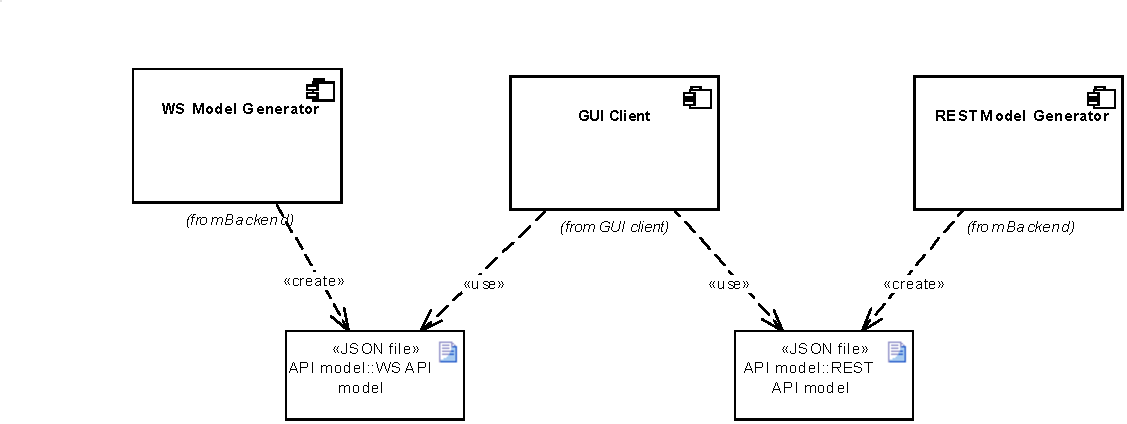
\includegraphics[width=13cm]{images-pdf/Architecture.pdf}
\caption{Architektura nástroje}
\label{fig:logo}
\end{center}
\end{figure}

Na 4 je znázorněna high-level architektura nástroje. Jsou zachyceny tři hlavní komponenty a
dva artefakty předávané mezi komponentami. Komponenty SOAP Maven plugin a REST
Maven plugin jsou popsány detailněji v 3.1.1, komponenta GUI klienta je podrobněji popsána
v 3.1.2. Pluginy jsou na sobě nezávislé a je tedy možné používat v projektu pouze jeden z
nich.

\subsection{Backend architektura}

Jelikož mají pluginy téměř identickou architekturu, je popisován pouze jeden z nich. Na 5 je
vidět diagram komponent pro REST plugin.

Význam a odpovědnost jednotlivých komponent:

Maven IoC Container

Komponenta reprezentující Maven proces, který pomocí dependency injection nakonfiguruje
a vytvoří instanci Maven REST Adapter.

\begin{figure}[h]
\begin{center}
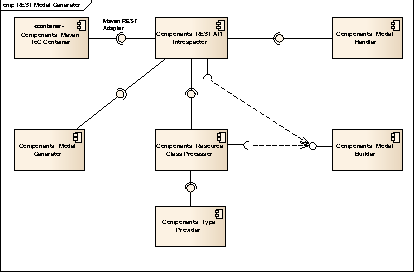
\includegraphics[width=13cm]{images-pdf/REST Model Generator.pdf}
\caption{Architektura pluginu pro REST služby}
\label{fig:logo}
\end{center}
\end{figure}

Maven REST Adapter

Komponenta sloužící jako wrapper pro předání řízení komponentě REST API Introspector.
Jedná se o návrhový vzor adapter, který zde slouží pro oddělení Maven API od funkcionality
pluginu. V budoucnu se může přidat adapter pro jiný buildovací nástroj než je Maven a
nebude nutné dělat žádný zásah do stávajícího zdrojového kódu.

Resource Class Processor

Komponenta provádějící introspekci REST API a JRAPIDoc anotací. Při introspekci jsou za
pomocí komponenty Model Builder vytvářeny části modelu, ze kterých se postupně tvoří
výsledný model.

Model Builder

Komponenta budující model. Komponenta obsahuje doménové třídy reprezentující model a
ke každé doménové třídě odpovídající builder třídu, která usnadňuje vytváření. Pro builder
třídy je použit návrhový vzor builder.

Type Provider

Tato komponenta se stará o zanesení informací o transportních typech do modelu. Řeší
problematiku popsanou v 2.4.3.3. Pomocí tovární metody je prováděna instanciace
konkrétního type providera, který se dále stará o samotnou funkcionalitu komponenty. Type
provider obsahuje cache, kde uchovává již prozkoumané typy, aby se nemusely opětovně
prohledávat. Cache také slouží jako úplný seznam typů, které se nakonec zakomponují do
modelu.

Model Handler

Uvnitř této komponenty se provádějí operace nad modelem definované v 2.4.3.4. Obsahuje
factory metodu provádějící instanciování nakonfigurovaných handlerů, které obsahují
naprogramované chování pro zpracování modelu. V komponentě jsou tyto handlery vykonány
a je zde i zpracování chyb vyskytujících se během provádění handlerů.

Model Generátor

Komponenta zodpovědná za vygenerování předaného modelu do souboru. Obsahuje také
konfiguraci způsobu serializace modelu.

\subsection{Architektura GUI klienta}

Pro návrh GUI klienta byl zvolen architektonický styl MVC (Model View Controller).
Přestože se jedná o jednoduchého klienta, budou z důvodu jednoduché rozšiřitelnosti a
přehlednosti vytvářeny komponenty a bude mezi ně rozdělena zodpovědnost.

\begin{figure}[h]
\begin{center}
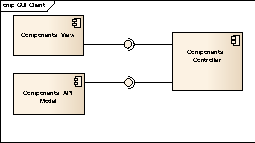
\includegraphics[width=13cm]{images-pdf/GUI-Client.pdf}
\caption{Architektura GUI klienta}
\label{fig:logo}
\end{center}
\end{figure}

Význam a odpovědnost jednotlivých komponent:

API Model

Komponenta zodpovědná za načtení modelu ze souboru a jeho uložení v ní.

View

Komponenta zodpovědná za zobrazování dat uživateli na obrazovce. Bude zobrazovat
grafickou podobu modelu, vyskytující se chyby (například při načítání modelu) apod.

Controller

Komponenta zodpovědná za inicializaci view i modelu. Obsahuje události vzniklé ve view a
funkcionalitu pro zaregistrování těchto událostí.

\section{Návrh API modelu}

Na 7 je znázorněn diagram tříd reprezentující model vzdáleného rozhraní, který vznikl na
základě analýzy v 2.4.3. Pro REST i WS služby bude existovat pouze jeden. Zda-li se vytvoří
instance reprezentace API k REST či WS bude záležet na řídící komponentě tvorby modelu,
která jej bude vytvářet.

\begin{figure}[h]
\begin{center}
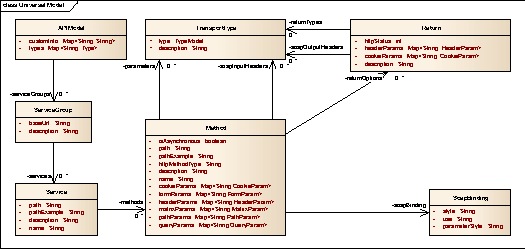
\includegraphics[width=13cm]{images-pdf/Universal-Model.pdf}
\caption{Model reprezentující vzdálené rozhraní}
\label{fig:logo}
\end{center}
\end{figure}

Popis tříd reprezentujících model:

APIModel

Hlavní kořenová třída obsahující tři hlavní atributy. První atribut customInfo reprezentuje
přídavné informace obdržené z konfigurace pluginu. Položky jsou vždy párové textové
řetězce klíč-hodnota. Následujícím atributem je seznam služeb sdružených ve skupinách
podle společné URI. Posledním atributem je seznam transportních typů ze všech skupin
služeb. Typy jsou zde vytvořeny na základě rekurzivního procházení každého typu a jeho
atributů.

ServiceGroup

Třída reprezentující skupinu služeb se stejným URI prefixem.

Service

Třída reprezentující kořenovou resource třídu (JAX-RS) nebo SEI (JAX-WS), která obsahuje
seznam svých metod.

Method

V JAX-RS kontextu třída reprezentuje jak resource metody kořenové resource třídy, tak i
rekurzivně obsažené metody resource tříd vrácených sub-resource lokátorem (podrobnosti v
2.2.2.4). Pro JAX-WS třída reprezentuje webovou operaci a obsahuje seznam vstupních
parametrů (JAX-RS může mít vždy jen jeden parametr). Při užití v JAX-WS má metoda
seznam vstupních SOAP hlaviček a seznam možností odpovědí. Seznam může být prázdný,
pokud je metoda JAX-WS jednosměrná.

SoapBinding

Třída nesoucí informace o způsobu serializování zpráv v kontextu JAX-WS.

Return

Třída nereprezentuje návratový typ metody jak evokuje její název, ale jednu možnou
odpověď, jakou může metoda vrátit. Odpověď se skládá z http statusu, návratových typů,
návratových typů SOAP hlaviček, seznamu http hlaviček a seznamu http cookie.

TransportType

Třída reprezentující transportní typ. Jejími atributy jsou popis transportního typu a datový typ
vytvořený type providerem (podrobněji v 2.4.3.3).

Návrh datových typů pro model znázorňuje diagram tříd 8. Návrh obsahuje tři možné typy:

\begin{figure}[h]
\begin{center}
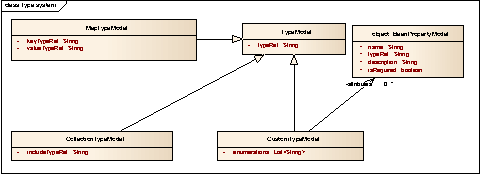
\includegraphics[width=13cm]{images-pdf/Type-System.pdf}
\caption{Reprezentace datových typů pro transport}
\label{fig:logo}
\end{center}
\end{figure}

CollectionTypeModel

Datový typ vycházející z Javovských kolekcí a polí. Obsahuje atribut nesoucí odkaz na typ,
jež je možné do kolekce či pole vložit. Může odkazovat na jakýkoliv typ, který je potomkem
třídy TypeModel.

MapTypeModel

Třída reprezentující Javovský datový typ Map<K, V>. Její atributy odkazují na datové typy,
jež reprezentují klíče a hodnoty, které mohou být do mapy vloženy. Mohou odkazovat na
jakýkoliv typ, který je potomkem třídy TypeModel.

CustomTypeModel

Třída reprezentuje datový typ běžných typů v Javě. Zahrnuje jak primitivní datové, tak i
objektové typy. Bude obsahovat všechny ostatní Javovské typy, které nepatří do skupin výše
zmíněných.

\section{Návrhové vzory}

Tato kapitola obsahuje popsané návrhové vzory jenž jsou použity v nástroji.

Factory method

\begin{figure}[h]
\begin{center}
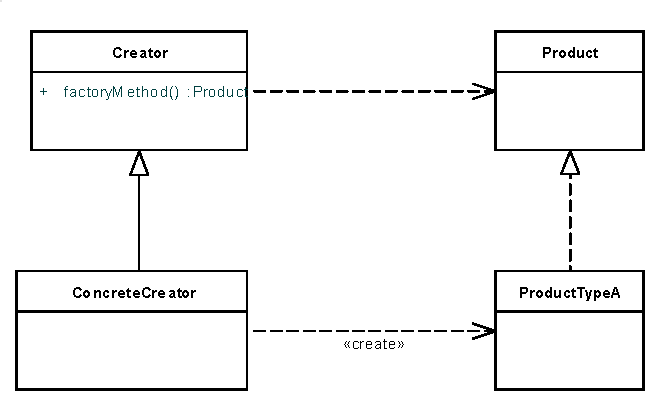
\includegraphics[width=13cm]{images-pdf/Factory-Method-Design-Patternnew.pdf}
\caption{Factory method pattern}
\label{fig:logo}
\end{center}
\end{figure}

Návrhový vzor patří do skupiny creational, která se zabývá principy pro 
vytváření objektů. Popisuje, jak vytvořit objekt bez použití konkrétní třídy. 
Tovární metodě jsou předány parametry, na základě kterých je rozhodnuto, ze 
které třídy bude vyrobena a vrácena instance. Je zde využito polymorfizmu, 
protože tovární metoda vrací instance tříd mající stejný nadtyp. Vzor tovární 
metoda je v nástroji použit v komponentách Model Handler a Type Provider 
popsaných v 3.1.1.

Builder

\begin{figure}[h]
\begin{center}
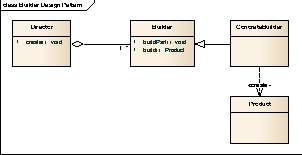
\includegraphics[width=13cm]{images-pdf/Builder-Design-Pattern.pdf}
\caption{Builder pattern}
\label{fig:logo}
\end{center}
\end{figure}

Návrhový vzor patřící také do skupiny creational vzorů a zabývající se 
principy vytváření objektů. Používá se pro konstrukci složitých objektů, 
kde se složité vytváření oddělí od reprezentace dat. Hlavní části v builder 
vzoru je vytvářený objekt, builder objekt obsahující funkcionalitu pro 
tvorbu vytvářeného objektu a director objekt, který řídí objekt builder 
a tím i celý proces tvorby objektu. Jakmile director ukončí vytváření objektu, 
zavolá na builder objektu metodu build, která vrátí vytvořený objekt. Vzor 
builder je použit pro tvorbu modelu a rekurzivně pro všechny jeho části. 
Model se nachází v komponentě Model Builder popsané v 3.1.1.

Adapter

\begin{figure}[h]
\begin{center}
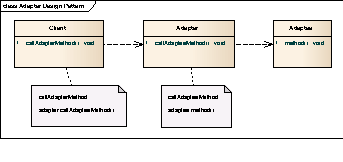
\includegraphics[width=13cm]{images-pdf/Adapter-Design-Pattern.pdf}
\caption{Adapter pattern}
\label{fig:logo}
\end{center}
\end{figure}

Návrhový vzor adapter patří do skupiny structural návrhových vzorů, jež se 
zabývají návrhem spojení mezi objekty. Používá se v případech, kdy existují 
dvě komponenty, ovšem nedokážou spolu komunikovat, protože vystavené rozhraní 
jedné komponenty je trochu jiné než požadované rozhraní druhé komponenty. Hrají 
zde roli objekty adaptovaný objekt, klient a adapter. V případech, kdy klient 
požaduje jiné rozhraní, než vystavuje adaptovaný, vloží se mezi klienta a 
adaptovaného objekt adapter. Ten bude zodpovědný za vystavení takového rozhraní 
klientovi a konzumování rozhraní adaptovaného, aby mohly komponenty mezi sebou 
komunikovat.

\chapter{Implementace}

\section{Použité technologie}

Java 6.0

Vyvíjený nástroj byl vyvíjen a kompilován do Java verze 6.0.

JAX-WS 2.0

Nástroj při vytváření modelu analyzuje kód JAX-WS specifikace ve verzi 2.0.

JAX-RS 2.0

Nástroj při vytváření modelu analyzuje kód JAX-RS specifikace ve verzi 2.0.

Apache Maven 3.3.1

Maven pluginy v nástroji byly vyvíjeny na verzích knihoven 3.3.1.

Reflections 0.9.9-RC2

Pro analýzu bytecode a vyhledání anotovaných tříd bylo použito Reflections ve verzi 0.9.9-
RC2.

Java Reflection API

Při analýze kódu bylo využito rozhraní Java Reflection API, jehož verze je vázaná k verzi
Javy.

Jackson 2.5.0

Knihovna ve verzi 2.5.0 použitá pro tvorbu transportních typů.

JUnit 4.11

Nástroj byl testován jednotkovými testy s použitím frameworku JUnit ve verzi 4.11.

Json2html

JavaScriptová knihovna zodpovědná za transformaci modelu v JSON formátu do HTML.
Transformace je prováděna na základě vytvoření šablony a její aplikace na JSON objekt.

\section{Vyhledávání JAX-WS a JAX-RS API}

Vyhledávání JAX-WS a JAX-RS spočívá ve vyhledání tříd majících anotace @Path a
@WebService, které jsou na classpath projektu. Zde jsou dvě možnosti jak třídy vyhledat.
První přístup je získání seznamu všech tříd na classpath a jejich postupné nahrávání do paměti
instancí třídy ClassLoader. Po nahrání třídy do paměti následně dotazování pomocí Java
Reflection API, zda třída obsahuje požadovanou anotaci. Tento přístup však není nejlepší
volbou především z hlediska časové náročnosti. V nejhorším případě budou muset být
nahrány všechny třídy, což může u většího projektu trvat desítky sekund. Nástroj používá
druhou metodu získání tříd, která je rychlejší. Třídy nejsou nahrávány do paměti, ale napřed
proběhne analýza bytecode a vyberou se pouze ty, které se do paměti nahrají. Poté jejich
nahrání je možné nad nimi používat Java Reflection API. Nástroj pro tento přístup používá
knihovnu Reflections, která je nástupcem knihovny Scannotation. Knihovně je třeba předat
instanci ClassLoaderu patřící k projektu a ne instanci, která patří k pluginu.

\section{Zpracování JAX-RS a JAX-WS API}

Ke zpracování vzdáleného rozhraní je použito Java Reflection API, pomocí kterého probíhá
analýza vytvořeného rozhraní. Rozhraní mohou obsahovat oproti klasickým třídám anotace a
datové typy z JAX-RS API, JAX-WS API a JRAPIDOC-API. Java Reflection API je
vlastností jazyka Java, která dokáže vykonávat nebo analyzovat sama sebe.

\section{Přídavné anotace}

Při použití specifikací pro tvorbu vzdáleného rozhraní nelze introspekcí kódu zjistit všechny
potřebné informace, které jsou definovány v požadavcích v kapitole 2.4. Jsou pro to
vytvořeny přídavné anotace, které mají za cíl pomoci tvořit detailnější dokumentaci. Anotace
jsou v samostatném balíku a lze je tedy volitelně připojit do projektu. Připojení probíhá
standardním přidáním Maven závislosti do projektu. Ani s použitím anotací nemusí být
dosaženo požadované dokumentace, protože by to mohlo vést k velmi složitému a
nepřehlednému anotování částí rozhraní. Vznikl proto kompromis, který je přehledný,
intuitivní a zároveň dokáže pokrýt většinu požadavků na tvorbu dokumentace.

Nově vzniklé anotace:

@org.jrapidoc.annotation.DocDescription

Přidává popis k elementům rozhraní.

@org.jrapidoc.annotation.rest.DocIsRequired

Indikuje zda je parametr či atribut povinný.

@org.jrapidoc.annotation.rest.DocPathExample

Protože v anotaci @Path mohou být regulární výrazy, které nemusejí být dobře čitelné, lze v
této anotaci uložit ukázku URI vyhovující regulárnímu výrazu.

@org.jrapidoc.annotation.rest.DocReturn

Anotace slouží k tvorbě možnosti odpovědi a je vytvořena především pro situace, kdy je
návratovým typem Response, ze kterého nelze při statické analýze získat žádné informace.

@org.jrapidoc.annotation.rest.DocReturns

Při více možnostech odpovědí lze možnosti vložit do této anotace.

@org.jrapidoc.annotation.soap.DocReturn

Pomáhá lépe zdokumentovat možnosti odpovědi.

@org.jrapidoc.annotation.soap.DocReturns

Při více možnostech odpovědí lze možnosti vložit do této anotace.

Další podrobnosti o přídavných anotacích lze nalézt v javadoc.

\section{Tvorba transportních typů}

Tvorba transportních typů může být prováděna buď zabudovanými třídami pro jejich tvorbu
nebo mohou být vytvořeny jiné třídy, které se nakonfigurují jako náhrada za původní
funkcionalitu. Defaultně se pro část REST používají třídy využívající knihovnu Jackson a pro
WS knihovna JAXB. V nástroji jsou ještě dvě třídy, které lze používat pro tvorbu
transportních typů. První z nich je kombinace Jackson a JAXB, Jackson je primární a JAXB
je sekundární. Druhou možností je také jejich kombinace, ale s obráceným pořadím. Výhodou
použití těchto zabudovaných tříd v nástroji je, že při tvorbě transportních typů jsou užity
anotace z těchto knihoven. Výsledný typ tedy bude odpovídat přesně tomu, jak jej bude
serializovat entity provider.

\chapter{Testování}

\section{Testování vývojářem}

Testování probíhalo paralelně s procesem vývoje. Cílem bylo ověřit, zda každá nově přidaná
část kódu provádí to, co se od ní čeká. Testování probíhalo připojením nástroje k Maven
projektu obsahujícímu JAX-RS a JAX-WS. Proces testování vývojářem probíhal provedením
buildu nástroje a následným spuštěním buildu testovaného projektu s módem debug. Maven
umožňuje mód debug spustit namísto běžného mvn příkazem mvnDebug, který otevře port a
čeká, dokud se debugger na tento port nepřipojí. Poté probíhá standardní debug Java aplikace.

\section{Jednotkové testy}

Jednotkové testy byly zaintegrovány do buildu nástroje, jejich vykonání a dosažené výsledky
tedy byly kontrolovány s každou novou tvorbou spustitelných balíčků. Cílem jednotkového
testování bylo provedení regresních testů. Pro měření kvality nástroje bylo vytvořeno přes sto
jednotkových testů.

\section{Integrační testy}

Integrační testování bylo realizováno zakomponováním pluginů nástroje do buildu
existujících projektů. Neslo si za cíl ověření chování pluginů a výsledek jejich výstupu.

Integrační testování bylo provedeno jak na testovacím projektu, tak na rozsáhlých existujících
projektech používajících pro tvorbu vzdálených rozhraní technologie JAX-RS a JAX-WS.

Prvním z existujících projektů byl projekt http://www.jbpm.org. jBPM je flexibilní balík pro
správu byznys procesů tvořící most mezi byznys analytiky a vývojáři. Produkt je dostupný
pod Apache Software License 2.0 a je zaštiťován firmou RedHat.

Druhým existujícím projektem byl Relationship Registry, jež slouží ke správě informací o
používaných nástrojích na projektech uvnitř společnosti CA Technologies. Vzhledem k tomu,
že se jedná o interní projekt, bylo integrační testování prováděno interním vývojářem
společnosti.

\section{Testování použitelnosti}

Cílová skupina

Znalost tvorby REST nebo WS na platformě JEE? Ano
Zkušenost s projekty spravovaném pomocí Maven? Ano
Zkušenost s přidáváním Maven pluginů do životního cyklu buildu? Ano

Cíle testování

Intuitivnost

Jedním z cílů testování je zjištění, jak je používání nástroje intuitivní. Uživatelé by neměli být
vystaveni neintuitivní konfiguraci. Naopak nástroj by měl mít možnost být spuštěn s
minimální konfigurací. Bude testováno, jak respondent využije pomocných funkcí a jestli mu
byly nápomocné. Pomocnými funkcemi je help goal v pluginu a javadoc rozhraní nástroje.

Přehlednost

Jelikož je nástroj možné různě rozšířit, bude testováno jestli se respondent bude v možnostech
rozšíření orientovat a podaří se mu takové rozšíření provést.

Provedení testů

Před provedením testů bude respondent seznámen se základními principy fungování nástroje a
poté mu budou předány scénáře pro provedení uživatelských akcí a adresář s klientem. Po
jejich vykonání mu budou vysvětleny rozšířené možnosti nástroje a předány další scénáře pro
provedení. Od respondenta bude požadováno komentování pozitivních, negativních poznatků
a komentování prováděných akcí ze scénářů. Celý průběh testování bude zaznamenán v audio
podobě.

\subsection{Testovací scénáře}

Vygenerování modelu pro JAX-RS

\begin{enumerate}
  \item Respondent připojí plugin do životního cyklu buildu.
  
  \item Respondent spustí goal help.
  
  \item Plugin vypíše informace o možnostech konfigurace.
  
  \item Respondent provede konfiguraci pluginu.
  
  \item Respondent spustí build projektu.
  
  \item Plugin vygeneruje do souboru model rozhraní.
  
  \item Respondent nalezne a otevře soubor s modelem.
\end{enumerate}

Načtení modelu v GUI klientovi

\begin{enumerate}
  \item Respondent nakopíruje do adresáře se zdroji GUI klienta.
  
  \item Respondent otevře ve webovém prohlížeči stránku s klientem.
  
  \item Načte se stránka.
  
  \item Respondent vloží adresu umístění modelu a stiskne „Load model“.
  
  \item Klient načte a zobrazí model.
  
Alternativní cesta:

  \item Pokud byla respondentem vložena neplatná cesta zobrazí se chybová hláška.
\end{enumerate}

Přidání popisu kořenové resource třídy

\begin{enumerate}
  \item Respondent přidá Maven závislost (org.jrapidoc:jrapidoc-annotation:1.0-SNAPSHOT)
do projektu
  \item Respondent přidá do kořenové resource třídy anotaci nacházející se v závislosti z
kroku 1

  \item Respondent spustí build projektu
  \item INCLUDE: Načtení modelu v GUI klientovi

  \item Respondent si zobrazí v modelu popis kořenové resource třídy
\end{enumerate}

\subsection{Výsledky}

Převážně v úvodu testování si respondent stěžoval na neexistující wiki stránku projektu.
Návod konfigurace pluginu se zdál být velmi stručný a pro člověka neznalého principů
fungování pluginu téměř nic neříkající. To by měla vyřešit wiki stránka, která by obsahovala
více podrobný popis konfigurace včetně jejích ukázek. Respondent navrhl, aby byl na wiki
také ukázkový projekt, na kterém by bylo vidět, jaké vlastnosti plugin má a jak se dá použít.

Ve scénářích není uvedeno, k jakému typu modulu se má plugin připojit. Respondent si tak
nebyl jistý, zda v multimodulovém projektu plugin připojit k modulu obsahující vzdálené
rozhraní nebo k war modulu, kde je rozhraní přidáno jako závislost. Nakonec se rozhodl
správně a připojil ho k war modulu.

Po seznámení se s nástrojem a představení jeho možností respondent ocenil funkce, kterými je
plná podpora atributů v resource třídách a podpora subresource lokátorů. Pozitivně hodnotil
také podporu WS a možnosti rozšíření nástroje nebo nahrazení komponent za vlastní.

Co se týče GUI klienta, na první pohled působí trochu nepřehledně, obzvlášť když uživatel při
procházení modelu neskrývá uzly, které již navštívil. Respondent navrhl provádět skrývání
automaticky za uživatele. Dalším poznatkem bylo umístění tlačítek pro nahrávání modelu a
pro přepínání mezi REST a WS.

Celkově nástroj zanechal působivý pocit z důvodů propracovanosti modelu a informací v něm
zanesených. Respondent má zkušenosti s používáním nástroje Swagger (popsán v 2.3.1) a po
seznámení se s novým nástrojem je ochotný přejít na používání nástroje JRAPIDoc. Většina
navržených změn byla provedena.

Ze zpětné vazby byl vytvořen ukázkový projekt, na kterém je demonstrováno použití nástroje.
Do GUI klienta byly aplikovány navržené změny pro lepší přehlednost a větší komfort
načítání modelů. Byla vytvořena wiki stránka na stránkách projektu.

\chapter{Srovnání}

Při srovnání nástrojů generujících dokumentaci ke vzdáleným rozhraním má nově vytvořený
nástroj mnohé co nabídnout oproti alternativám. Při tvorbě nástroje bylo myšleno na pozitiva
a negativa konkurenčních nástrojů popsaných v 2.3.

Co se týče porovnání tvorby dokumentace REST služeb na platformě Java EE, byl nástroj
především srovnáván s nástrojem Swagger. Ten je v současné době nejpopulárnějším
nástrojem na tvorbu dokumentace pro REST služby. Nástroj se od Swaggeru a dalších
odlišuje kombinací plné podpory specifikace JAX-RS a otevřeným kódem. Nástroj se také
snaží být jednoduchý na konfiguraci a ovládání na rozdíl od Swagger, který obsahuje poměrně
velkou a pro začátečníka nesrozumitelnou konfiguraci.

\section{Konfigurace}

Pokud chceme provést konfiguraci Maven pluginu je dobré si ji zobrazit pomocí spuštění
goalu help u konkrétního pluginu. Při spuštění goalu pro Swagger plugin s parametrem
-Ddetail=true se žádné informace nezobrazí a volání skončí vyhozenou výjimkou
NullPointerException. Plugin nástroje Miredot goal pro zobrazení konfigurace ani
neobsahuje, tudíž nelze získat vůbec žádné informace. Nástroj JRAPIDoc oproti
ostatním při spuštění zobrazí očekávanou nápovědu konfigurace.

Při srovnání samotné konfigurace se jako nejobtížnější jeví ta ve Swaggeru. Miredot a
JRAPIDoc mají konfiguraci stručnou a snadno pochopitelnou. Swagger umožňuje
integrovat dva různé GUI klienty, kde každý je v pom.xml konfigurován pomocí
jiných elementů. To působí při prvním kontaktu s nástrojem velmi zmatečně,
protože například ani nevíme o existenci druhého a pokud konfigurujeme jiného
než jsme si stáhli, není nám jasné proč konfigurace nebyla aplikována.

\section{Podpora JAX-RS API}

Nástroj Swagger po úspěšné konfiguraci a následném pokusu o vygenerování modelu
dokumentace nic nevygeneruje. Swagger tvoří model jen u tříd a metod, které
jsou anotovány jeho přídavnými anotacemi. U tříd a metod je vždy nutné
duplikovat hodnotu z JAX-RS anotace @Path do anotace Swaggeru. Takové řešení je
problematické, když nemůžeme upravovat zdrojový kód tříd rozhraní. To může
nastat, pokud jsou třídy do projektu přidány jako knihovny. S touto vlastností
Swaggeru je spojena ještě jedna nevýhoda. Tou je nutnost modifikace kódu při změně seznamu
dokumentovaných tříd. JRAPIDoc je flexibilnější, po nakonfigurování pluginu automaticky vyhledá třídy rozhraní.
Ty jsou vyhledávány v určených Java balíčcích. Může se stát, že v balíčku jsou i třídy, které
dokumentovat nechceme. Taková funkčnost je řešena za pomocí konfigurace, ve
které se vydefinuje seznam tříd k vynechání. Pokud nastane situace, kdy v jednom
buildu je nutné vygenerovat více než jednu dokumentaci, se Swaggerem se to
nepodaří, protože je vždy nutný zásah do zdrojového kódu.

Pokud jsou v třídě rozhraní přítomny atributy, které jsou anotovány pomocí 
@MatrixParam, @CookieParam a @FormParam, Swagger je v dokumentaci
nezobrazí. Stejný problém nastane i při použití anotací nad setter metodami
atributů. Po spuštění JRAPIDoc jsou v dokumentaci atributy injektované všemi
definovanými anotacemi (@MatrixParam, @CookieParam, @FormParam, @QueryParam,
@PathParam a @HeaderParam) z JAX-RS. Je také možné injektovat parametry
konstruktoru, tuto vlastnost podporuje nástroj JRAPIDoc, Swagger nikoliv.

Výše zmíněnými anotacemi lze injektovat i jiné datové typy než jsou Java
primitivní typy a String (viz \ref{ch:atributy}). Runtime provádí převod na tyto
typy z datového typu String, tudíž v dokumentaci by se měl objevit datový
typ String a ne ten, který vznikne transformací v runtime.
Swagger ovšem do dokumentace vygeneruje datové typy až po převodu ze String, což
není korektní. JRAPIDoc korektně vygeneruje informaci o datovém typu.

Ve specifikaci je definováno dynamické rozhodování obsluhy požadavku a slouží
pro to tzv. sub-resource lokátory. Podrobnější informace o sub-resource
lokátorech jsou popsány v \ref{subsec:resource-metoda}. JRAPIDoc takové chování
plně podporuje narozdíl od Swagger. Ten se k sub-resource lokátorům chová jako
by se jednalo o resource metodu. Pokud jsou v rozhraní použity sub-resource
lokátory výsledkem Swaggeru je vypsání chyby a není zobrazena dokumentace
ani k ostatním metodám a rozhraním.

JAX-RS specifikuje dědičnost tříd, se vzdáleným rozhraním, algoritmem popsaným v
\ref{subsec:dedicnost-resource-trid}. Swagger tento nevyužívá a dědičnost tříd
ignoruje. Anotace definované v nadtřídách a interfacech jsou ignorovány. I přes
přidání Swagger anotací do třídy předka a potomka metoda v dokumentaci zahrnuta
není. JRAPIDoc takto definovaný algoritmus pro průchod předky aplikuje při
introspekci kódu a výsledkem je model dokumentace, který odpovídá navrženému rozhraní.








V kontextu SOAP webových služeb na platformě Java EE se nepodařilo najít alternativu pro
srovnání nástroje. Výsledkem této práce je tak pravděpodobně první nástroj svého druhu,
který v sobě obsahuje možnost tvorby dokumentace pro WS. Tvorba dokumentace pro REST
i WS při použití jednoho nástroje má tu výhodu, že dokumentace je sjednocená jak po
grafické, tak po obsahové stránce.
a

a

aa

a

aa

a

aa

a

aa

a

aa

a

aa

a

aa

a

aa

a

aa

a

aa

a

aa

a

aa

a

aa

a

aa

a

aa

a

aa

a

aa

a

aa

a

aa

a

aa

a

aa

a

aa

a

a

\chapter{Budoucí práce}

Bylo by možné přidat volitelně generování modelu do jiných formátů než je JSON a do jiných
specifikací modelu než používá nástroj defaultně. Například by mohlo jít o podporu
serializace stávající struktury modelu do XML formátu či podporu transformace a
vygenerování modelu do WADL. Jelikož nástroj poskytuje rozhraní pro přidání rozšiřujících
operací, nebyla by nutná změna v kódu nástroje, ale stačilo by pouze implementovat a přidat
operaci do konfigurace pluginu.

Následujícím možným rozšířením by mohla být podpora dalších technologií umožňujících
vzdálenou komunikaci v Javě EE. Vedle podpory REST a WS by tak mohla jednou z
takových technologií být JMS.

Momentálně nástroj nepodporuje XML jmenné prostory, které se používají v JAX-WS. Do
budoucna by mohla přibýt podpora volitelně je do modelu přidat.

\chapter{Závěr}

Diplomová práce si kladla za cíl navržení, implementování a otestování nástroje pro tvorbu
dokumentace vzdáleného rozhraní na technologiích JAX-WS a JAX-RS. Důležitou
prerekvizitou samotné tvorby nástroje bylo zanalyzování principů tvorby vzdáleného rozhraní
především pak na platformě Java EE. Nástroj byl vyvinut jako zásuvný modul do Apache
Maven. Pro tvorbu dokumentace projektu obsahujícího Java třídy se vzdáleným rozhraním je
postačující nástroj napojit do životního cyklu buildu a provést základní konfiguraci. Pro
kvalitnější a podrobnější dokumentaci je možné do kódu rozhraní přidat pomocné prvky ve
formě Java anotací, které byly vytvořeny jako doplněk k Maven pluginům.

Po závěrečné fázi realizace byly na nástroji provedeny integrační a uživatelské testy.
Výsledky z těchto testů byly vzaty v potaz a byly zakomponovány do nástroje.

Cíl práce se podařilo splnit podle zadání. Nástroj navíc poskytuje rozhraní, které umožňuje do
nástroje doplnit vlastní operace nad modelem rozhraní. Dále je možné některé komponenty
nahradit za jiné.

Nástroj a jeho zdrojový kód je uvolněn pod open-source svobodnou licencí a bude integrován
do projektu jBPM.

\chapter{Reference}
a

a

aa

a

aa

a

aa

a

aa

a

aa

a

aa

a

aa

a

aa

a

aa

a 

aa

a

a

%*****************************************************************************

% M. Dušek radi:
%\bibliographystyle{alpha}
% kdy citace ma tvar [AutorRok] (napriklad [Cook97]). Sice to asi neni  podle ceske normy (BTW BibTeX stejne neodpovida ceske norme), ale je to nejprehlednejsi.
% 3.5.2009 JZ polemizuje: BibTeX neobvinujte, napiste a poskytnete nam styl (.bst) splnujici citacni normu CSN/ISO.

%*****************************************************************************
%*****************************************************************************
\appendix

\chapter{Seznam použitých zkratek}
a

a

aa

a

aa

a

aa

a

aa

a

aa

a

aa

a

aa

a

aa

a

aa

a

aa

a

aa

a

aa

a

aa

a

aa

a

aa

a

aa

a

aa

a

aa

a

a

\chapter{Instalační a uživatelská příručka} 
a

a

aa

a

aa

a

aa

a

aa

a

aa

a

aa

a

aa

a

aa

a

aa

a

aa

a

aa

a

aa

a

aa

a

aa

a

aa

a

aa

a

aa

a

aa

a

a

\chapter{Obsah přiloženého CD}

\end{document} 